\newcommand{\dicty}{\emph{D.~discoideum}}

% gene names
\newcommand{\nlp}{\emph{\mbox{nlp-31}}}
\newcommand{\ftna}{\emph{\mbox{ftn-1}}}
\newcommand{\ftnb}{\emph{\mbox{ftn-2}}}
\newcommand{\cysl}{\emph{\mbox{cysl-1}}}
\newcommand{\nog}{\emph{\mbox{nog-1}}}
\newcommand{\nhr}{\emph{\mbox{nhr-57}}}
\newcommand{\lam}{\emph{\mbox{lam-3}}}

\newcommand{\fog}{\emph{\mbox{fog-2(lf)}}}
\newcommand{\egl}{\emph{\mbox{egl-9}(lf)}}
\newcommand{\rhy}{\emph{\mbox{rhy-1}(lf)}}
\newcommand{\vhl}{\emph{\mbox{vhl-1}(lf)}}
\newcommand{\eglvhl}{\emph{\mbox{egl-9(lf);vhl-1(lf)}}}
\newcommand{\eglhif}{\emph{\mbox{egl-9(lf)}~\mbox{hif-1(lf)}}}
\newcommand{\hif}{\emph{\mbox{hif-1(lf)}}}

% protein names
\newcommand{\eglp}{EGL-9}
\newcommand{\rhyp}{RHY-1}
\newcommand{\nogp}{NOG-1}
\newcommand{\vhlp}{VHL-1}
\newcommand{\hifp}{HIF-1}
\newcommand{\fogp}{FOG-2}
\newcommand{\nhrp}{NHR-57}
\newcommand{\lamp}{LAM-3}
\newcommand{\cyslp}{CYSL-1}

% DE genes numbers:
\newcommand{\egln}{1,806}
\newcommand{\rhyn}{2,103}
\newcommand{\vhln}{689}
\newcommand{\eglvhln}{2,376}
\newcommand{\hifn}{546}
\newcommand{\eglhifn}{404}
\newcommand{\fogn}{2090}
\newcommand{\total}{5,671} % isoforms!!!!
% \newcommand{\inall}{53}
% \newcommand{\allup}{10}
% \newcommand{\alldown}{13}

% downstream targets
\newcommand{\egltargets}{126}
\newcommand{\rhytargets}{0}
\newcommand{\vhltargets}{45} % 44 genes, minus vhl-1 (IDed due to deletion)
\newcommand{\hiftargets}{195}
\newcommand{\hifohtargets}{31}


% website commands
\newcommand{\website}{
            \url{https://wormlabcaltech.github.io/Angeles_Leighton_2016/}
            }
\newcommand{\webref}{
\href{https://wormlabcaltech.github.io/Angeles_Leighton_2016/}{website}}

% more space between rows
\newcommand{\ra}[1]{\renewcommand{\arraystretch}{#1}}

\section*{Abstract}
\textbf{
RNA-seq is commonly used to identify genetic modules that respond to perturbations.
In single cells, transcriptomes have been used as phenotypes, but this concept
has not been applied to whole-organism RNA-seq. Linear models can quantify
expression effects of individual mutants and identify epistatic effects in double
mutants. However, interpreting these high-dimensional measurements is unintuitive.
We developed a single coefficient to quantify transcriptome-wide epistasis which
accurately reflects the underlying interactions. To demonstrate the power of our
approach, we sequenced four single and two double C. elegans mutants. From these
mutants, we successfully reconstructed the known hypoxia pathway. Using this
approach, we uncovered a class of 31 genes that have opposing changes in expression
in \egl{} and \vhl{} but the \eglvhl{} mutant phenocopies \egl{}.
These changes violate the classical model of HIF-1 regulation, but can be explained
by postulating a role of hydroxylated HIF-1 in transcriptional control.
}
\vspace{10mm}


\section*{Introduction}
\label{sec:introduction}
Genetic analysis of molecular pathways has traditionally been performed
through epistatis analysis. Generalized epistasis indicates that two genes interact
functionally; such interaction can involve the direct interaction of their
products or the interaction of any consequence of their function (small molecules,
physiological or behavioral effects)~\citep{Huang2006}. If two
genes interact, and the mutants of these genes have a quantifiable phenotype,
the double mutant of interacting genes will have a phenotype that is not the sum
of the phenotypes of the single mutants that make up its genotype. Epistasis
analysis remains a cornerstone of genetics today~\citep{Phillips2008}.


Recently, biological studies have shifted in focus from studying single
genes to studying all genes in parallel. In particular,
RNA-seq~\citep{Mortazavi2008} enables biologists to
identify genes that change expression in response to a perturbation. Gene expression
profiling using RNA-seq has become much more sensitive thanks to deeper and more
frequent sequencing due to lower sequencing costs~\citep{Metzker2010},
better and faster abundance quantification~\citep{Patro2014,Bray2016,Patro2015},
and improved differential expression analysis
methods~\citep{Pimentel2016,Trapnell2013}. RNA-seq has been
successfully used to identify genetic modules involved in a variety of processes,
including T-cell regulation~\citep{Singer2016,Shalek2013}, the
\emph{Caenorhabditis~elegans} (\cel{}) linker
cell migration~\citep{Schwarz2012}, and planarian stem cell
maintenance~\citep{VanWolfswinkel2014,Scimone2014}. For the most part, the role of
transcriptional profiling has been restricted to target gene identification.

Although transcriptional profiling has been primarily used for descriptive purposes,
transcriptomic phenotypes have previously been used to make genetic inferences.
Microarray analyses in \emph{S. cerevisiae} and \dicty{} were used to show
that transcriptomes can be interpreted to infer genetic relationships in simple
eukaryotes~\citep{Hughes2000, VanDriessche2005}.\@ eQTL studies in
many organisms, from yeast to humans, have established the usefulness of
transcriptomic phenotypes for population genetics studies~\citep{Brem2002,Schadt2003,
Li2006,King2014}. In cell culture, single-cell RNA-seq has seen significant
progress towards using transcriptomes as phenotypes with which to test genetic
interactions~\citep{Adamson2016,Dixit2016}.
More recently, we have identified a new developmental state
of \cel{} using whole-organism transcriptome profiling~\citep{Angeles-Albores2016a}.
To investigate the ability of whole-organism transcriptomes to serve as quantitative
phenotypes for epistasis analysis in metazoans, we sequenced the transcriptomes of
of four well-characterized loss of function mutants in the \cel{} hypoxia
pathway~\citep{Epstein2001,Shen2006,Shao2009,Jiang2001}.

% carmie:
Metazoans depend on the presence of oxygen in sufficient concentrations to
support aerobic metabolism. Genetic pathways evolved to rapidly respond to any
acute or chronic changes in oxygen levels at the cellular or organismal level.
Biochemical and genetic approaches identified the Hypoxia Inducible Factors
(HIFs) as an important group of oxygen-responsive genes that are involved in a
broad range of human pathologies~\citep{Semenza2012}.

Hypoxia Inducible Factors are highly conserved in metazoans~\citep{Loenarz2011}.
A common mechanism for hypoxia-response induction is heterodimerization between a
HIF$\alpha$ and a HIF$\beta$ subunit; the heterodimer then initiates
transcription of target genes~\citep{Jiang1996}. The number and complexity of
HIFs varies throughout metazoans, with humans having three HIF$\alpha$ subunits
and two HIF$\beta$ subunits, whereas in the roundworm \cel{} there is a single
HIF$\alpha$ gene, \gene{hif-1}~\citep{Jiang2001} and a single HIF$\beta$
gene, \gene{ahr-1}~\citep{Powell-Coffman1998}. HIF target genes have been implicated
in a wide variety of cellular and extracellular processes including glycolysis,
extracellular matrix modification, autophagy and immunity~\citep{Semenza1994,
Bishop2004,Shen2005,Bellier2009,Semenza2012}.

Levels of HIF$\alpha$ proteins tend to be tightly regulated. Under conditions of
normoxia, \hifp{}$\alpha$ exists in the cytoplasm and partakes in a futile cycle
of continuous protein production and rapid degradation~\citep{Huang1996}.
\hifp{}$\alpha$ is hydroxylated by three proline hydroxylases
in humans (PHD1, PHD2 and PHD3) but is only hydroxylated by one proline
hydroxylase (\eglp{}) in \cel{}~\citep{Kaelin2008}. \hifp{} hydroxylation
increases its binding affinity to Von Hippel Lindau Tumor Suppressor 1
(\vhlp{}), which allows ubiquitination of \hifp{} leading to its subsequent
degradation. In \cel{}, \eglp{} activity is inhibited by binding of \cyslp{},
and \cyslp{} activity is in turn inhibited at the protein level by \rhyp{},
possibly by post-translational modifications to \cyslp{}~\citep{Ma2012} (see
Fig.~\ref{fig:pathway}).

% heatmap
\begin{figure}[tbhp]
\centering
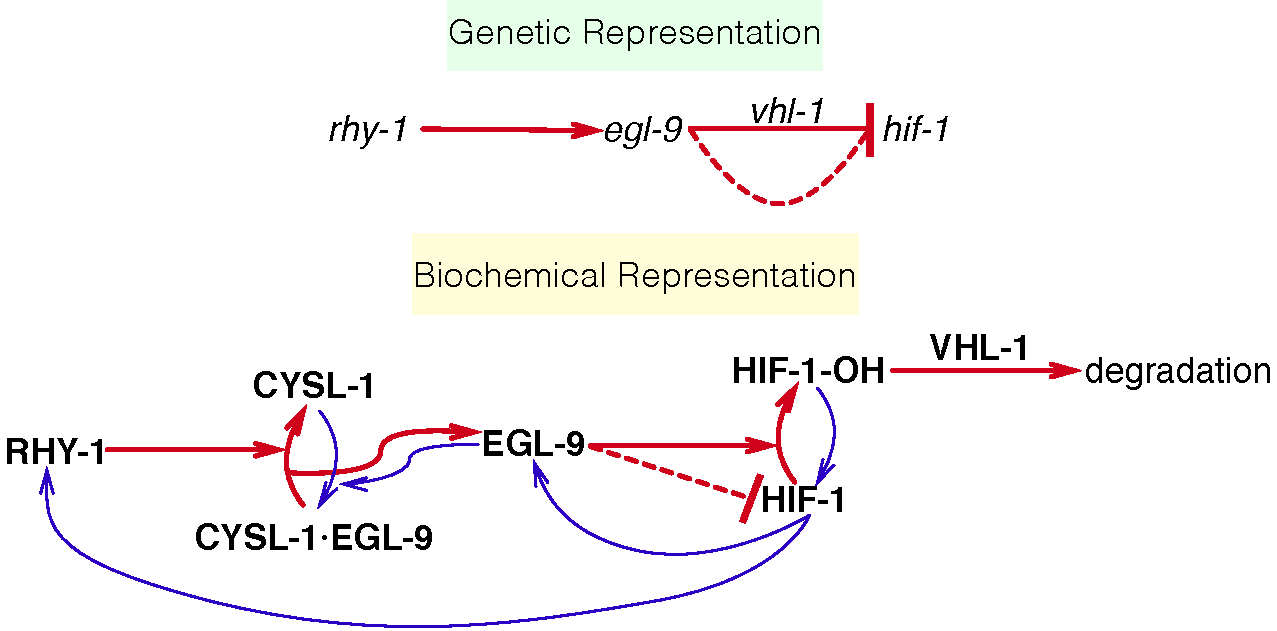
\includegraphics[width=.7\linewidth]{hypims/HIF1pathway.pdf}
\caption{
Genetic and biochemical representation of the hypoxia pathway in \cel{}.
Red arrows are arrows that lead to inhibition of \hifp{}, and blue arrows
are arrows that increase \hifp{} activity or are the result of \hifp{} activity.
\eglp{} is known to exert \gene{vhl-1}-dependent and independent repression
on \hifp{} as shown in the genetic diagram. The \gene{vhl-1}-independent
repression of \hifp{} by \eglp{} is denoted by a dashed line and is not dependent
on the hydroxylating activity of \eglp{}.
Technically, RHY-1 inhibits CYSL-1, which in turn inhibits EGL-9, but this
interaction was abbreviated in the genetic diagram for clarity.
}
\label{fig:pathway}
\end{figure}

Here, we show that transcriptomes contain robust signals that can be
used to infer relationships between genes in complex metazoans by reconstructing
the hypoxia pathway in \cel{} using RNA-seq.
Furthermore, we show that the phenomenon of phenotypic epistasis, a hallmark of
genetic interaction, holds at the molecular systems level.
We also demonstrate that transcriptomes contain sufficient information, under
certain circumstances, to order genes in a pathway using only single mutants.
Finally, we were able to identify genes that appear to be downstream of \gene{egl-9}
and \gene{vhl-1}, but do not appear to be targets of \gene{hif-1}.
Using a single set of genome-wide measurements, we were able to observe and
quantitatively assess  significant fraction of the known transcriptional
effects of \gene{hif-1} in \cel{}.
A complete version of the analysis, with ample documentation, is available at
\url{https://wormlabcaltech.github.io/mprsq}.

\section*{Results}
\subsection*{The hypoxia pathway controls thousands of genes in \cel{}}
\label{sub:summary}

We selected four single mutants within the hypoxia pathway for expression profiling:
\egl{} (\emph{sa307}), \rhy{} (\emph{ok1402}), \vhl{} (\emph{ok161}), \hif{} (\emph{ia4}).
We also sequenced the transcriptomes of two double mutants, \eglvhl{} (\emph{sa307},
\emph{ok161}) and \eglhif{} (\emph{sa307}, \emph{ia4}) as well as wild-type N2 as
a control sample. Each genotype  was sequenced in triplicate at a depth of 15
million reads. We performed whole-organism RNA-seq of these mutants at a moderate
sequencing depth ($\sim7$ million mapped reads for each individual replicate)
under normoxic conditions. For single samples, we identified around 22,000 different
isoforms per sample, which allowed us to measure differential expression of 18,344
isoforms across all replicates and genotypes (this constitutes  $\sim$70\% of
the protein coding isoforms in \cel{}).
We also included in our analysis a \fog{} (\emph{q71}) mutant which we have previously
studied~\citep{Angeles-Albores2016a}, because \gene{fog-2} is not reported to
interact with the hypoxia pathway.
We analyzed our data using a general linear model on
logarithm-transformed counts. Changes in gene expression are reflected in the
regression coefficient, $\beta$ which is specific to each isoform within a genotype.
Statistical significance is achieved when the q-values for each $\beta$ (p-values
adjusted for multiple testing) are less than 0.1. Genes that are significantly
altered between wild-type and a given mutant have $\beta$ values that are
statistically significantly different from 0.  These coefficients are not equal
to the average log-fold change per gene, although they are loosely related to
this quantity. Larger magnitudes of $\beta$ correspond to larger perturbations.
These coefficients can be used to study the RNA-seq data in question.

In spite of the moderate sequencing depth, transcriptome profiling of the hypoxia
pathway revealed that this pathway controls thousands of genes in \cel{}. The
\egl{} transcriptome showed differential expression of \egln{} genes. Similarly,
\rhyn{} genes were differentially expressed in \rhy{} mutants. The \vhl{}
transcriptome showed considerably fewer differentially expressed genes (\vhln{}),
possibly because it is a weaker controller of \hif{} than
\egl{}~\citep{Shao2009}. The \egl{};\vhl{} double mutant transcriptome showed
\eglvhln{} differentially expressed genes. The \hif{} mutant also showed a
transcriptomic phenotype involving \hifn{} genes. The \eglhif{} double mutant
showed a similar number of genes with altered expression (\eglhifn{} genes, see
Table~\ref{tab:genes}).

\begin{table}[tbhp]
  \centering
  \begin{tabular}{lr}
    \toprule{}
    Genotype & Differentially Expressed Genes \\
    \midrule{}
    \egl{} & \egln{}\\
    \rhy{} & \rhyn{}\\
    \vhl{} & \vhln{}\\
    \eglvhl{} & \eglvhln{}\\
    \eglhif{} & \eglhifn{}\\
    \fog{} & \fogn{}\\
    \bottomrule{}
  \end{tabular}
  \caption{Number of differentially expressed genes in each mutant.}
\label{tab:genes}
\end{table}

\subsection*{Principal Component Analysis visualizes epistatic relationships between genotypes}
\label{sub:Clustering}

Principal Component Analysis (PCA) is a well-known technique in bioinformatics that is
used to identify relationships between high dimensional data points~\citep{Yeung2001}
We performed PCA on our data to examine whether each genotype clustered in a biologically
relevant manner. PCA identifies the vector that can explain most of the variation
in the data;this is called the first PCA dimension. Using PCA, one can identify
the first $n$ dimensions that can explain more than 95\% of the variation in the
data. Sample clustering in these $n$ dimensions often indicates biological
relationships between the data, although interpreting PCA dimensions can be
difficult.

After applying PCA, we expected \hif{} to cluster near \eglhif{}, because
\hif{} exhibits no phenotypic defects under normoxic conditions, in contrast to
\egl{}, which exhibits an egg-laying (Egl) phenotype in the same environment.
In \eglhif{} mutants the Egl phenotype of \egl{} mutants is suppressed and instead
the grossly wild-type phenotype of \hif{} is observed. On the other hand, we
expected \egl{}, \rhy{}, \vhl{} and \eglvhl{} to form a separate cluster since
each of these genotypes is Egl and has a constitutive hypoxic response. Finally,
we included as a negative control a \fog{} mutant we have analyzed
previously~\citep{Angeles-Albores2016a}. This data was obtained at a different
time from the other genotypes, so we included a batch-normalization term in our
equations to account for this. Since \gene{fog-2} has not been described
to interact with the hypoxia pathway, we expected that it should appear far away
from either cluster.

The first dimension of the PCA analysis was able to discriminate between mutants
that have constitutive high levels of \hifp{} and mutants that have no \hifp{},
whereas the second dimension was able to discriminate between mutants within the
hypoxia pathway and outside the hypoxia pathway (see Fig.~\ref{fig:pca}).
Therefore expression profiling measures enough signal to cluster genes in a
meaningful manner in complex metazoans.

\begin{figure}[tbhp]
\centering
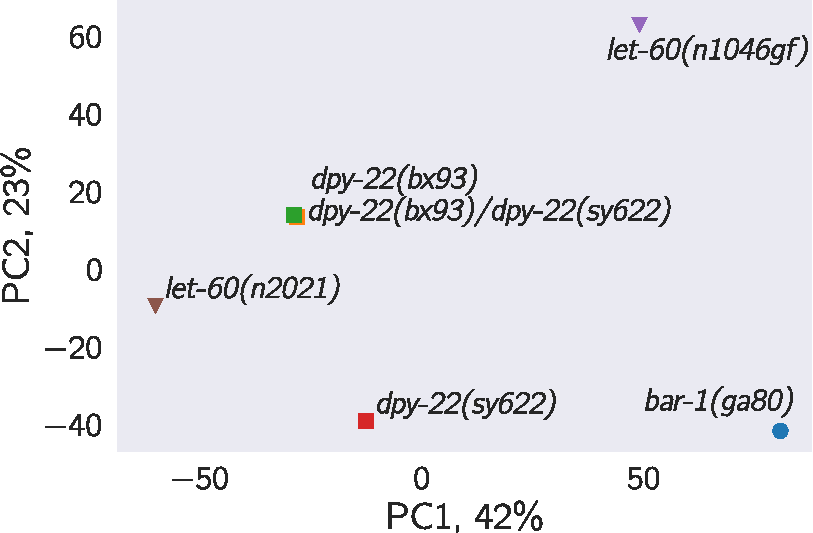
\includegraphics[width=0.5\linewidth]{hypims/pca.pdf}
\caption{
Principal component analysis of various \cel{} mutants. Genotypes that have an
activated hypoxia response (\emph{i.e}, \egl{}, \vhl{}, and \rhy{}) cluster far
from \hif{}. \hif{} clusters with the suppressed \eglhif{} double mutant.
The \fog{} transcriptome, used as an outgroup, is far away from either cluster.
}
\label{fig:pca}
\end{figure}

\subsection*{Reconstruction of the hypoxia pathway from first genetic principles}
\label{sec:reconstruct}
Having shown that the signal in the mutants we selected was sufficient to
cluster mutants using the values of the regression coefficients $\beta$, we set
out to reconstruct the hypoxia pathway from genetic first principles. In general,
to reconstruct a pathway, we must first assess whether two genes act on the same
phenotype. If they do not act on the same phenotype (the set of commonly differentially
regulated genes between two mutants is empty), these mutants are independent.
If they are not independent, then two mutants have a shared transcriptomic
phenotype (STP)---a set of genes or isoforms that are differentially expressed in
both mutants, without taking into account what direction they change in. In this
case, we must measure whether these genes act additively or epistatically on the
measured phenotype; if there is epistasis we must measure whether it is
positive or negative, in order to assess whether the epistatic relationship is a
genetic suppression or a synthetic interaction.

\subsubsection*{Genes in the hypoxia mutant act on the same transcriptional phenotype}
\label{sec:phenotypes}
We observed that all the hypoxia mutants had significant shared transcriptomic
phenotypes (fraction of the transcriptomes that was shared between mutants
ranged from a minimum of 6.8\% shared between \hif{} and \eglvhl{} to a maximum
of 31\% shared genes between \egl{} and \eglvhl{}). For comparison, we also
analyzed a previously published \fog{} transcriptome~\citep{Angeles-Albores2016a}.
The \gene{fog-2} gene is involved in masculinization of the \cel{} germline,
which enables sperm formation, and is not known to be involved in the hypoxia
pathway. The hypoxia pathway mutants and the \fog{} mutant also showed shared
transcriptomic phenotypes (3.6\%--12\% genes), but correlations between
expression level changes were considerably weaker (see below), suggesting that
there is minor cross-talk between these pathways.


% genetic correlations
\begin{figure}[tbhp]
\centering
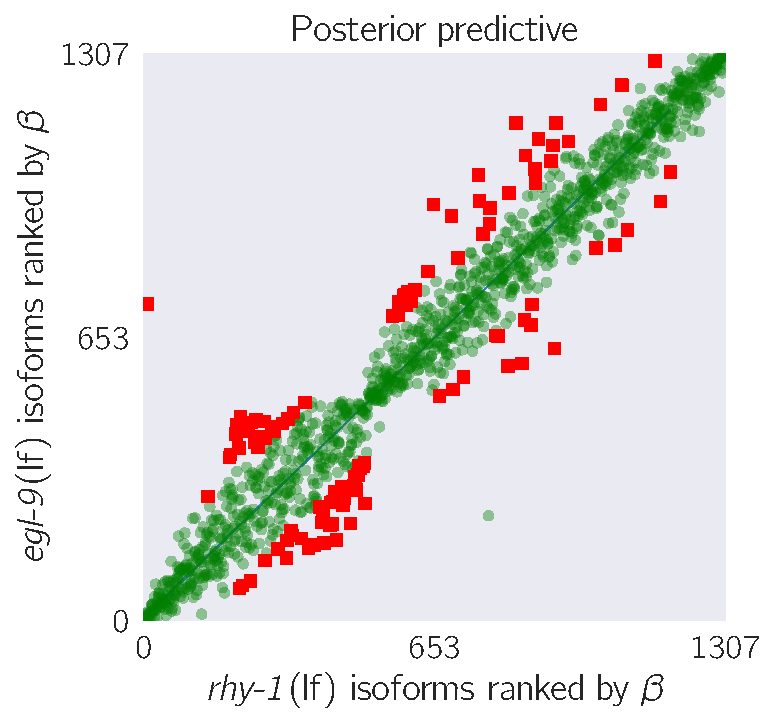
\includegraphics[width=.4\linewidth]{hypims/multiplemodes-eb.pdf}
\caption{
Strong transcriptional correlations can be identified between genes
that share a positive regulatory connection. We took the \egl{} and the \rhy{}
transcriptomes, identified differentially expressed genes common to both
transcriptomes and ranked each gene according to its differential expression
coefficient $\beta$. We plotted the rank of each gene in \rhy{} versus the
rank of the same gene in the \egl{} transcriptome. The result is an almost
perfect correlation. Green, transparent large points mark inliers to the primary
regressions (blue lines); red squares mark outliers to the primary regressions.
}
\label{fig:genetic_interactions}
\end{figure}

We wanted to know whether it was informative to look at quantitative agreement
within STPs. For each mutant pair, we rank-transformed
the regression coefficients $\beta$ of each isoform within the STP, and
calculated lines of best fit using Bayesian regression with a Student-T
distribution to mitigate noise from outliers and plotted the results in a rank plot
(see Fig~\ref{fig:genetic_interactions}). For transcriptomes associated with the
hypoxia pathway, we found that these correlations tended to have
values higher than 0.9 with a tight distribution around the line of best fit.
The correlations for mutants from the hypoxia pathway
with the \fog{} mutant were considerably weaker, with magnitudes between
0.6--0.85 and greater variance around the line of best fit.
Although \gene{hif-1} is known to be genetically repressed by \gene{egl-9}, \gene{rhy-1} and
\gene{vhl-1}~\citep{Epstein2001,Shen2006}, all the correlations
between mutants of these genes and \hif{} were positive.

After we calculated the pairwise correlation within each STP,
we weighted the result of each regression by the
number of isoforms within the STP and
divided by the total number of differentially expressed isoforms present in the
two mutant transcriptomes that contributed to that specific STP,
$N_\mathrm{overlap}/N_{\mathrm{g_1} \cup \mathrm{g2}}$.
The weighted regressions recapitulated a module network (see Fig.~\ref{fig:heatmap}).
We identified a strong positive interaction between \egl{} and \rhy{}.
The magnitude of this weighted correlation derives from the magnitude of the
transcriptomes for these mutants (\egln{} and \rhyn{} differentially expressed
genes respectively) and the overlap between both genes was
extensive, which makes the weighting factor considerably larger than other pairs.
The weak correlation between \hif{} and \egl{} results from the small size of
the \hif{} transcriptome and the small overlap between the transcriptomes.

The fine-grained nature of transcriptional phenotypes means that these weighted
correlations between transcriptomes of single mutants are predictive of genetic
interaction.

% heatmap
\begin{figure}[tbhp]
\centering
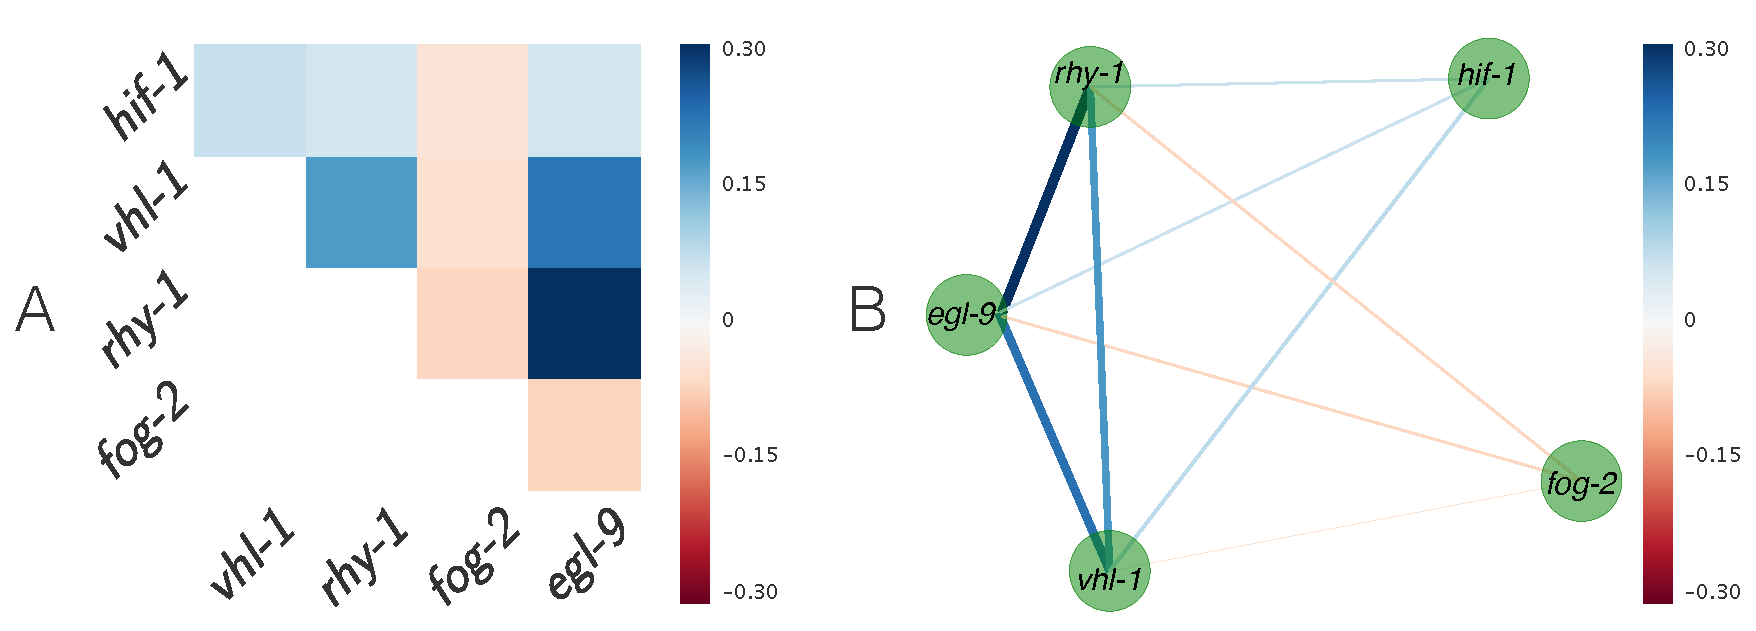
\includegraphics[width=\linewidth]{hypims/bayesian-heatmap-horizontal.pdf}
\caption{
\textbf{A}. Heatmap showing pairwise regression values between all
single mutants. \textbf{B}. Correlation network drawn from \textbf{A}. Edge
width is proportional to the logarithm of the magnitude of the weighted
correlation between two nodes divided by absolute value of the weighted
correlation value of smallest magnitude. Edges are also colored according to the
heatmap in \textbf{A}. Inhibitors of \gene{hif-1} are tightly correlated and form
a control module;
\gene{hif-1} is positively correlated to its inhibitors, albeit weakly;
and
\gene{fog-2}, a gene that is not reported to interact with the hypoxia pathway,
has the smallest, negative correlation to any gene.
}
\label{fig:heatmap}
\end{figure}

\subsubsection*{A quality check of the transcriptomic data reveals excellent agreement
            with the literature}
\label{sub:quality_check}
One way to establish whether genes are acting additively or epistatically to each
other is to perform qPCR of a reporter gene in the single and double mutants. This
approach was used to successfully map the relationships within the hypoxia
pathway (see, for example~\citep{Shao2009,Shen2006}). A commonly used hypoxia reporter
gene is \nhr{}, which is known to exhibit a several-fold increase in mRNA
expression when \hifp{} accumulates~\citep{Shen2006,Shen2005,Park2012}. Likewise,
increased \hifp{} fucntion is known to cause increased of \gene{rhy-1}
and \gene{egl-9}~\citep{Powell-Coffman2010}.

We can
selectively look at the expression of a few genes at a time. Therefore, we
queried the changes in expression of \gene{rhy-1}, \gene{egl-9}, and \nhr{}. We
included the nuclear laminin gene \lam{} as a representative negative control not
believed to be responsive to alterations in the hypoxia pathway.
\nhr{} was upregulated in \egl{}, \rhy{} and \vhl{}, but remains unchanged in \hif{}.
\eglvhl{} had an expression level similar to \egl{}; whereas the
\eglhif{} mutant showed wild-type levels of the reporter expression, as reported
previously~\citep{Shen2006} (see Fig.~\ref{fig:qpcr}).

% in silico qPCR
\begin{figure}[tbhp]
\centering
\includegraphics[width=.5\linewidth]{hypims/qpcr.pdf}
\caption{
\textbf{Top}: Observed $\beta$ values of select genes. We selected
four genes (\gene{rhy-1}, \gene{egl-9}, \nhr{} and \lam{}, shown on the x-axis)
and plotted their regression coefficients, $\beta$, as measured for every
genotype (represented by one of six colors) to study the epistatic relationships
between each gene. Asterisks above a bar represent a regression coefficient
statistically significantly different from 0 (\qval{1}) relative to a wild-type
control. Error bars show standard error of the mean
value of $\beta$. \nhr{} is an expression reporter that has been used previously
to identify \gene{hif-1} regulators~\citep{Shen2006,Shao2009}. \lam{} is shown here
as a negative control that should not be altered by mutations in this pathway.
We measured modest increases in the levels of \gene{rhy-1} mRNA when \hif{} is
knocked out.
}
\label{fig:qpcr}
\end{figure}

We observed changes in \rhy{} expression consistent with previous
literature~\citep{Shen2006} when \hifp{} accumulates.
We also observed increases in \gene{egl-9} expression in \egl{}.
\gene{egl-9} is known as a hypoxia responsive gene~\citep{Powell-Coffman2010}.
Although changes in \gene{egl-9} expression were not statistically significantly
different from the wild-type in
\rhy{} and \vhl{} mutants, the mRNA levels of \gene{egl-9} still trended towards
increased expression in these genotypes.
As with \nhr{}, \gene{egl-9} and \gene{rhy-1} expression were wild-type in
\eglhif{} and \eglvhl{} mutant showed expression phenotypes identical to \egl{}.
This dataset also showed that knockout of \gene{hif-1} resulted in a modest
increase in the levels of \gene{rhy-1}. This suggests that \gene{hif-1}, in
addition to being a positive regulator of \gene{rhy-1}, also inhibits it, which
constitutes a novel observation.
Using a single reporter we would have been able to reconstruct an
important fraction of the genetic relationships between the genes in the hypoxia
pathway–--but would likely fail to observe yet other genetic interactions, such as
the evidence for \gene{hif-1} negatively regulating \gene{rhy-1} transcript levels.


\subsection*{Transcriptome-wide epistasis}
Ideally, any measurement of transcriptome-wide epistasis should conform to certain
expectations. First, it should make use of the regression coefficients of as
many genes as possible. Second, it should be summarizable in a single,
well-defined number. Third, it should have an intuitive behavior, such that
special values of the statistic should each have an unambiguous interpretation.

One way of displaying transcriptome-wide epistasis is to plot transcriptome data onto
an epistasis plot (see Fig~\ref{fig:egl9epistasis}). In an epistasis plot, the
X-axis represents the expected expression of a double mutant $a^-b^-$ if $a$
and $b$ interact additively.
In other words, each individual isoform's x-coordinate is the sum of the regression
coefficients from the single mutants $a^-$ and $b^-$.
The Y-axis represents the deviations from the additive (null) model, and
can be calculated as the difference between the observed regression coefficient
and the predicted regression coefficient. Only genes that are differentially
expressed in all three genotypes are plotted. Assuming that the two genes interact
via a simple phenotype (for example, if both genes affect a transcription factor
that generates the entire transcriptome), these plots will generate specific
patterns that can be described through linear regressions. The slope of these
lines, $s_{a,b}$, is the transcriptome-wide epistasis coefficient.

Epistasis plots can be understood intuitively for simple cases of genetic
interactions. If two genes act additively on the same set of differentially expressed
isoforms then all the plotted points will fall along the line $y=0$.
If two genes interact in an unbranched pathway, then $a^-$ and $b^-$ should
have identical phenotypes for $a^-$, $b^-$ and $a^-b^-$, if all the genotypes are
homozygous for genetic null alleles~\citep{Huang2006}. It follows that the
data points should fall along a line with slope equal to $-\frac{1}{2}$. On the
other hand, in the limit of complete inhibition of $a$ by $b$, the plots should show
a line of best fit with slope equal to $-1$\footnote{Specifically, this follows
from assuming that $b^-$ is wild-type under the conditions assayed; and
$a^-b^-$ = $b^-$ = wild-type}.
Genes that interact synthetically (\emph{i.e.}, through an OR-gate) will fall
along lines with slopes $>0$. When there is epistasis of one gene over another,
the points will fall along a line of best fit with slope $s_{ab=b}$ or $s_{ab=a}$.
This slope must be determined from the single-mutant data.
From this information, we can use the single mutant data to predict the
distribution of slopes that results for each case stated above, as well as for
each epistatic combination ($a^-b^-=a^-$ or $a^-b^-=b^-$). The transcriptome-wide
epistasis coefficient ($s_{a, b}$), emerges as a powerful way to quantify epistasis
because it integrates information from many different genes or isoforms into a
single number (see Fig.~\ref{fig:egl9epistasis}).

In our experiment, we studied two double mutants, \eglhif{} and \eglvhl{}.
We wanted to understand how well an epistasis analysis based on transcriptome-wide
coefficients agreed with the epistasis results reported in the literature, which
were based on qPCR of single genes. Therefore, we performed orthogonal distance
regression on the two gene combinations we studied (\gene{egl-9} and
\gene{vhl-1}; and \gene{egl-9} and \gene{hif-1}) to determine the epistasis
coefficient for each gene pair. We also generated models for the special cases
mentioned above (additivity, $a^-b^-=a^-$, strong suppression, etc\ldots) using
the single mutant data. For every simulation, as well as for the observed data,
we used bootstraps to generate probability distributions of the epistasis
coefficients.

When we compared the predictions for the transcriptome-wide epistasis coefficient,
$s_{egl-9,vhl-1}$ under different assumptions with the observed slope ($-0.42$). We
observed that the predicted slope matched the simulated slope for the case where
\gene{egl-9} is epistatic over \gene{vhl-1} (\egl{} = \eglvhl{}, see
Fig.~\ref{fig:egl9epistasis}) and did not overlap with any other prediction.
Next, we predicted the distribution of $s_{egl-9,hif-1}$ for different pathways
and contrasted with the observed slope. In this case, we saw that the uncertainty
in the observed coefficient overlapped significantly with the strong suppression
model, where \eglp{} strongly suppresses \hifp{}, and also with the model where
\hif{} = \eglhif{}. In this case, both models are reasonable---\hifp{} is strongly
suppressed by \eglp{}, and we know from previous literature that the epistatic
relationship, \hif{} = \eglhif{}, is true for these mutants. In fact, as the
repression of \hifp{} by \eglp{} becomes stronger, the epistatic model should converge
on the limit of strong repression (see
\href{https://wormlabcaltech.github.io/mprsq/analysis_notebooks/epistasis_6.html}
{Epistasis}).

Another way to test which model best explains the epistatic relationship between
\gene{egl-9} and \gene{vhl-1} is to use Bayesian model selection to calculate
an odds ratio between two models to explain the observed data. Models can be placed
into two categories: parameter-free and fit. Parameter free models are `simpler'
because their parameter space is smaller (0 parameters) than the fit models ($n$
parameters). By Occam's razor, simpler models should be preferred to more
complicated models. However, simple models suffer from the drawback that
systematic deviations from them cannot be explained or accomodated, whereas more
complicated models can alter the fit values to maximize their explanatory power.
In this sense, more complicated models should be preferred when the data shows
systematic deviations from the simple model. Odds-ratio selection gives us a way
to quantify the trade-off between simplicity and explanatory power.

We reasoned that comparing a fit model ($y = \alpha\cdot x$, where $\alpha$ is
the slope of best fit) against a parameter-free model ($y = \gamma\cdot x$,
where $\gamma$ is a single number) constituted a conservative approach towards
selecting which theoretical model (if any) best explained the data. In particular,
this approach will tend to strongly favor the line of best fit over simpler model
for all but very small, non-systematic deviations. We decided
that we would reject the theoretical models only if the line of best-fit
was $10^3$ times more likely than the theoretical models (odds ratio, OR $>10^3$).
Comparing the odds-ratio between the line of best fit and the different pathway
models for \gene{egl-9} and \gene{vhl-1} showed similar results to the simulation.
Only the theoretical model \egl{} = \eglvhl{} could not be rejected (OR = 0.46),
whereas all other models were significantly less likely than the line of best fit
(OR $>10^{44}$).
Therefore, \gene{egl-9} is epistatic to \gene{vhl-1}. Moreover,
since $s_{egl-9, vhl-1}$ is strictly between and not equal to $0$ and $-0.5$, we
conclude that \gene{egl-9} acts on its transcriptomic phenotype in
\gene{vhl-1}-dependent and independent manners. A branched pathway that can lead
to epistasis coefficients in this range is a pathway where \gene{egl-9} interacts
with its transcriptomic phenotype via branches that have the same valence (both
positive or both negative)~\citep{Shao2009}. When we performed a similar analysis
to establish the epistatic relationship between \gene{egl-9} and \gene{hif-1},
we observed that the best alternative to a free-fit model was a model where
\gene{hif-1} is epistatic over \gene{egl-9} (OR$=2551$), but the free-fit model
was still preferred. All other models were strongly rejected (OR $>10^{25}$).

% epistasis graph
\begin{figure}[tbhp]
\centering
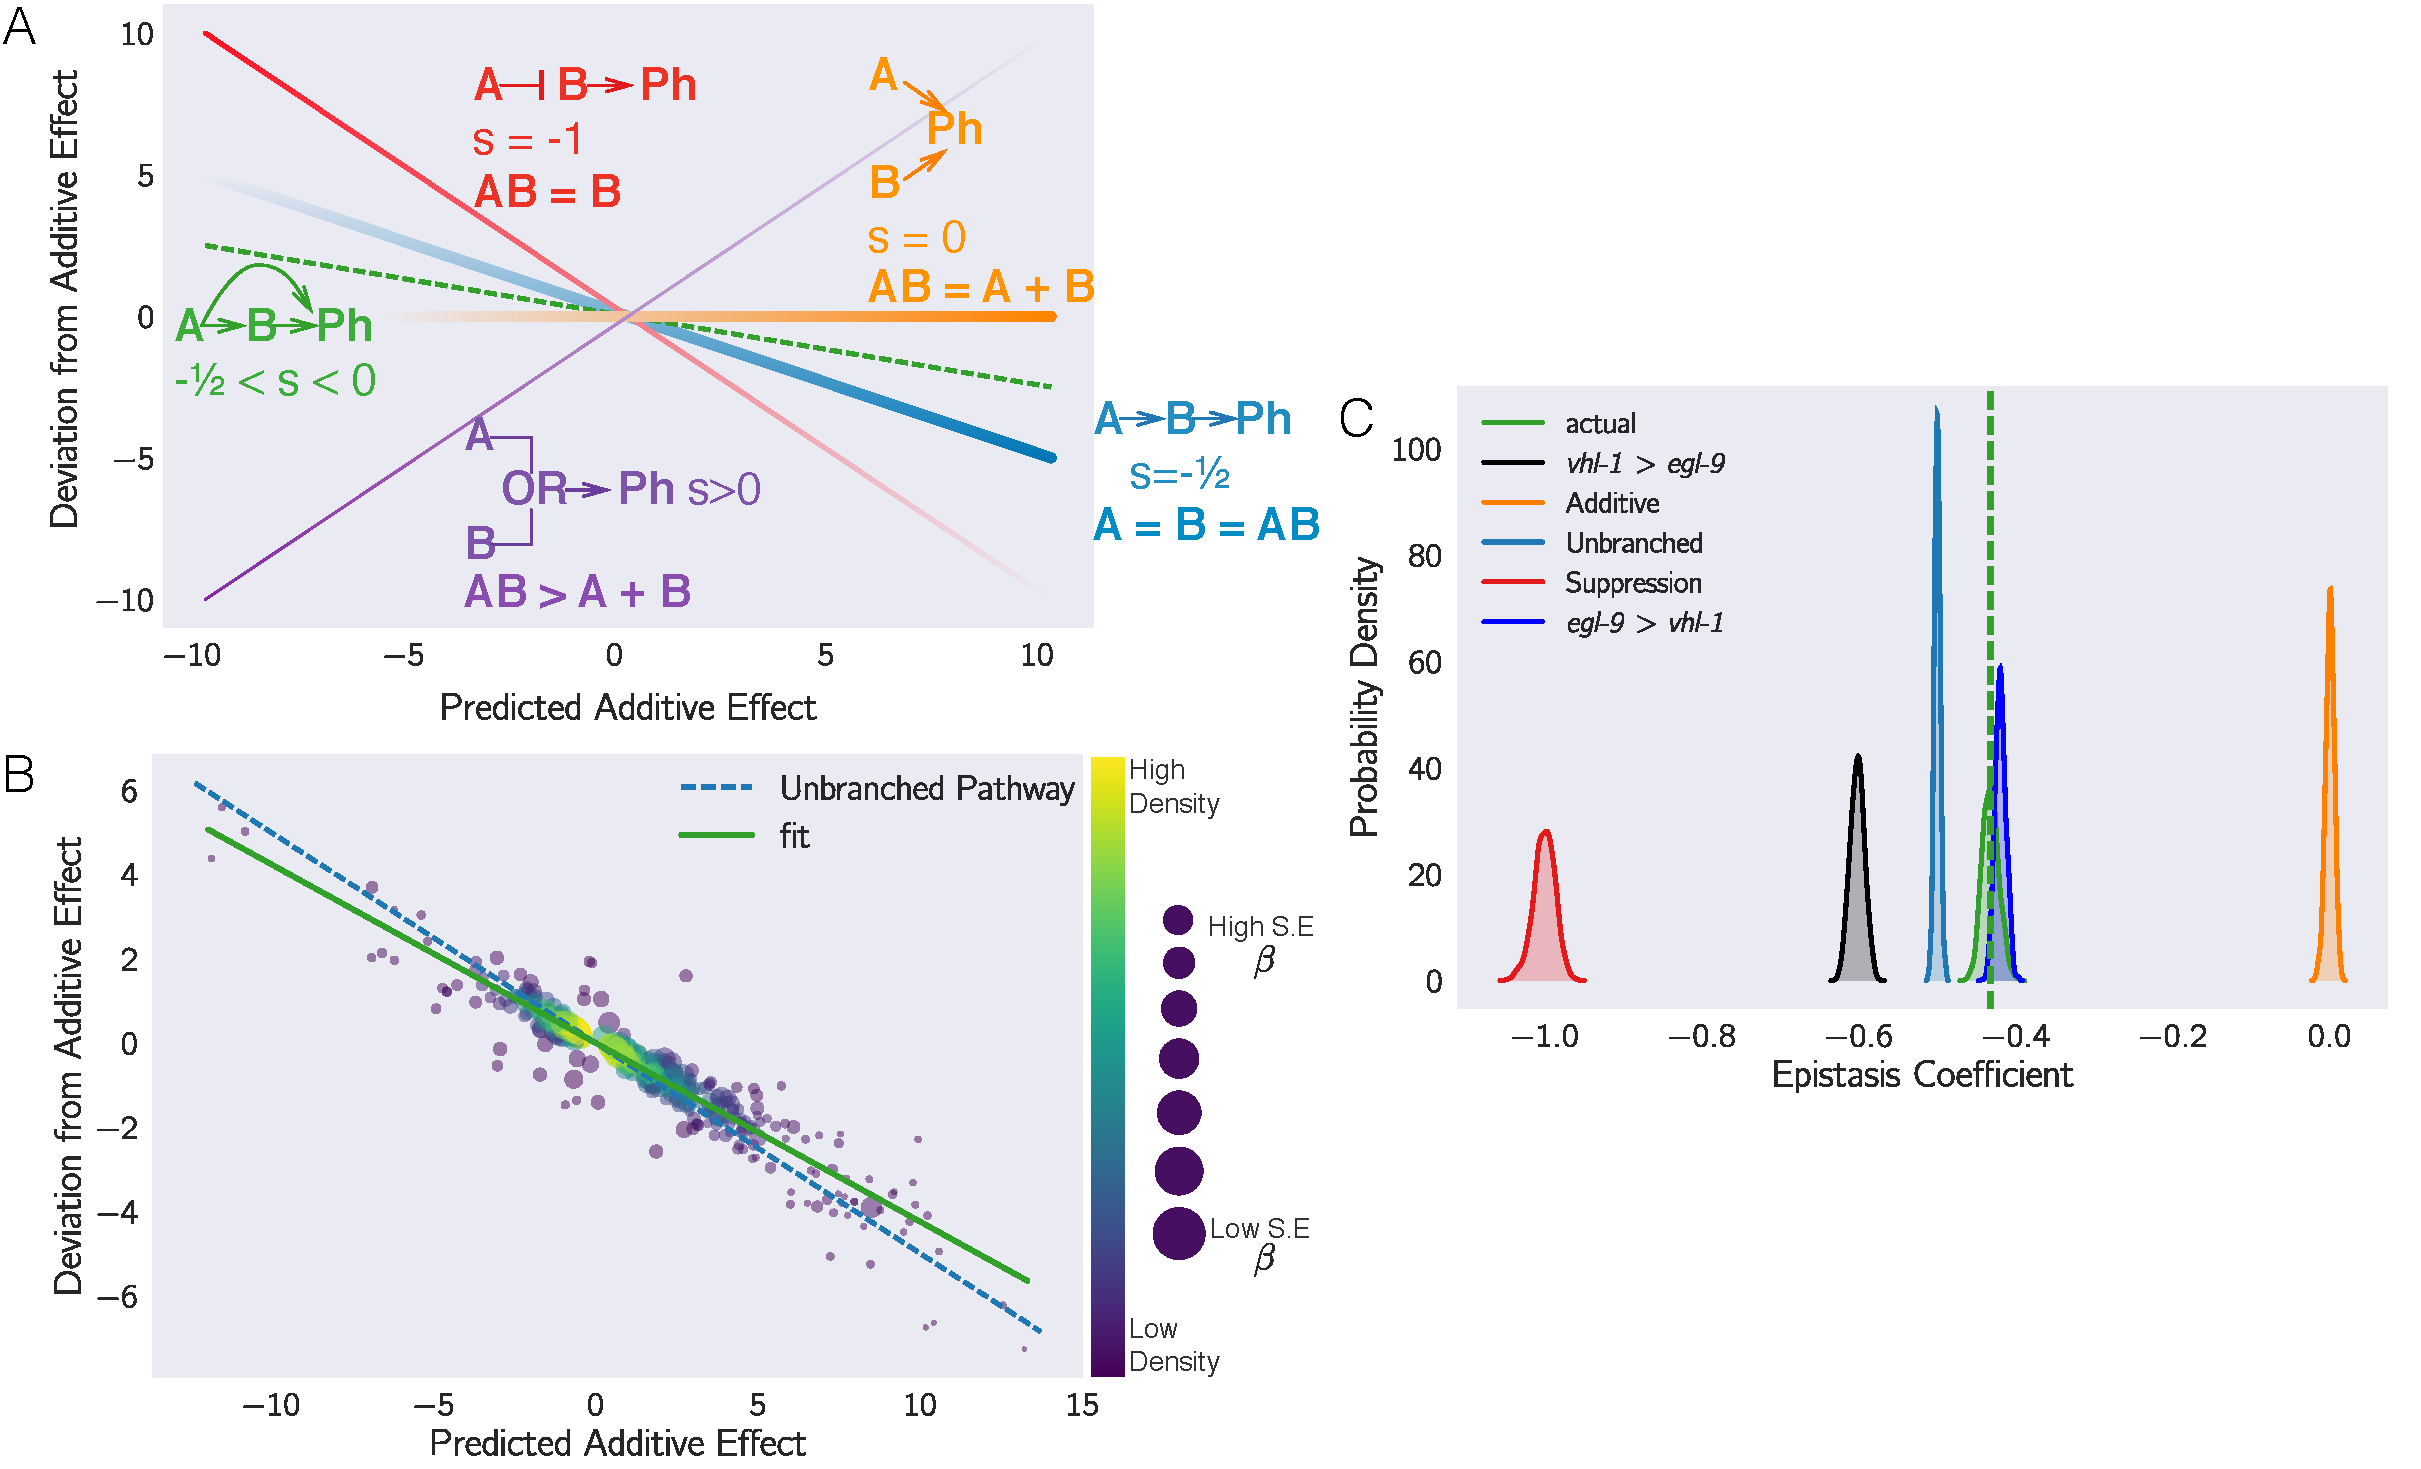
\includegraphics[width=\linewidth]{hypims/egl9hif1-epistasis-horizontal.pdf}
\caption{
(\textbf{A}) Schematic diagram of an epistasis plot. The X-axis on an epistasis
plot is the expected coefficient for a double mutant under an additive model
(null model). The Y-axis plots deviations from this model. Double mutants that
deviate in a systematic manner from the null model exhibit transcriptome-wide epistasis
($s$). To measure $s$, we perform a linear regression on the data. The slope of
the line of best fit is $s$. This coefficient is related to genetic architectures.
Genes that act additively on a phenotype \textbf{(Ph)} will have $s=0$ (orange
line); whereas
genes that act along an unbranched pathway will have $s=-1/2$ (blue line).
Strong
repression is reflected by $s=-1$ (red line). Cases where $s>0$ correspond to
synthetic interactions (purple line), and in the limit as $s\rightarrow\infty$,
the synthetic interaction
must be an OR-gate. Cases where $0 < s < -1/2$ correspond to circuits
that have multiple positive branches; whereas cases where
$-1/2<s< -1$ correspond to cases where the branches have different valence.
Cases where $s < -1$ represent inhibitory branches.
(\textbf{B}) Epistasis plot showing
that the \eglvhl{} transcriptome deviates significantly from a null additive.
Points are colored qualitatively according to density (purple---low,
yellow---high) and size is inversely proportional to the standard
error (S.E.) of the y-axis (larger points, higher accuracy). The purple line
is the line of best fit from an orthogonal distance regression.
(\textbf{C}) Comparison of simulated epistatic coefficients against the observed
coefficient. Green curve shows the bootstrapped observed transcriptome-wide epistasis
coefficient for \gene{egl-9} and \gene{vhl-1}. Dashed green line shows the mean
value of the data. Using the single mutants, we simulated coefficient
distributions for a linear model (light blue, centered at $-0.5$);
an additive model (orange, centered at 0); a model where either
\gene{egl-9} or \gene{vhl-1} masks the other phenotype (dark blue and black,
respectively) and a complete suppression model (red, centered at $-1$).
The observed coefficient overlaps the predicted epistasis curve for
\eglvhl{} = \egl{} (green and dark blue).
}
\label{fig:egl9epistasis}
\end{figure}

\subsubsection*{Epistasis can be predicted}
Given our success in measuring epistasis coefficients, we wanted to know whether
we could predict the epistasis coefficient between \gene{egl-9} and \gene{vhl-1}
in the absence of the \egl{} genotype. Since \rhyp{} indirectly activates
\eglp{}, the \rhy{} transcriptome should contain more or less
equivalent information to the \egl{} transcriptome. Therefore, we generated
predictions of the epistasis coefficient between \gene{egl-9} and \gene{vhl-1}
by substituting in the \rhy{} data. We predicted $s_{rhy-1,vhl-1} = -0.45$.
Similarly, we used the \eglvhl{} double mutant to
measure the epistasis coefficient while replacing the \egl{} dataset with the \rhy{}
dataset. We found that the epistasis coefficient using this substitution was $-0.40$.
This coefficient was different from $-0.50$ (OR $>10^{62}$), reflecting the same
qualitative conclusion that the hypoxia pathway is branched.
In conclusion, we were able to obtain a quantitatively close prediction of the
epistasis coefficient for two mutants using the transcriptome of a related,
upstream mutant. Finally, we showed that in the absence of a single mutant, an
upstream locus can under some circumstances be used to estimate epistasis
between two genes.


\subsection*{Transcriptomic decorrelation can be used to infer functional distance}
\label{sub:decorrelation}
% What are functional interactions?
So far, we have shown that RNA-seq can accurately measure genetic interactions.
However, genetic interactions are far removed from biochemical interactions:
Genetic interactions do not require two gene products to interact physically, nor
even to be physically close to each other. RNA-seq cannot measure physical
interactions between genes, but we wondered whether expression profiling contains
sufficient information to order genes along a pathway.

Single
genes are often regulated by multiple independent sources. The connection between
two nodes can in theory be characterized by the strength of the edges connecting
them (the thickness of the edge); the sources that regulate both
nodes (the fraction of inputs common to both nodes); and the genes that are
regulated by both nodes (the fraction of outputs that are common to both nodes).
In other words, we expected that expression profiles associated with a pathway
would respond quantitatively to quantitative changes in activity of the pathway.
Targeting a pathway at multiple points would lead to expression profile
divergence as we compare nodes that are separated by more degrees of freedom,
reflecting the flux in information between them.

% decorrelation
\begin{figure}[tbhp]
\centering
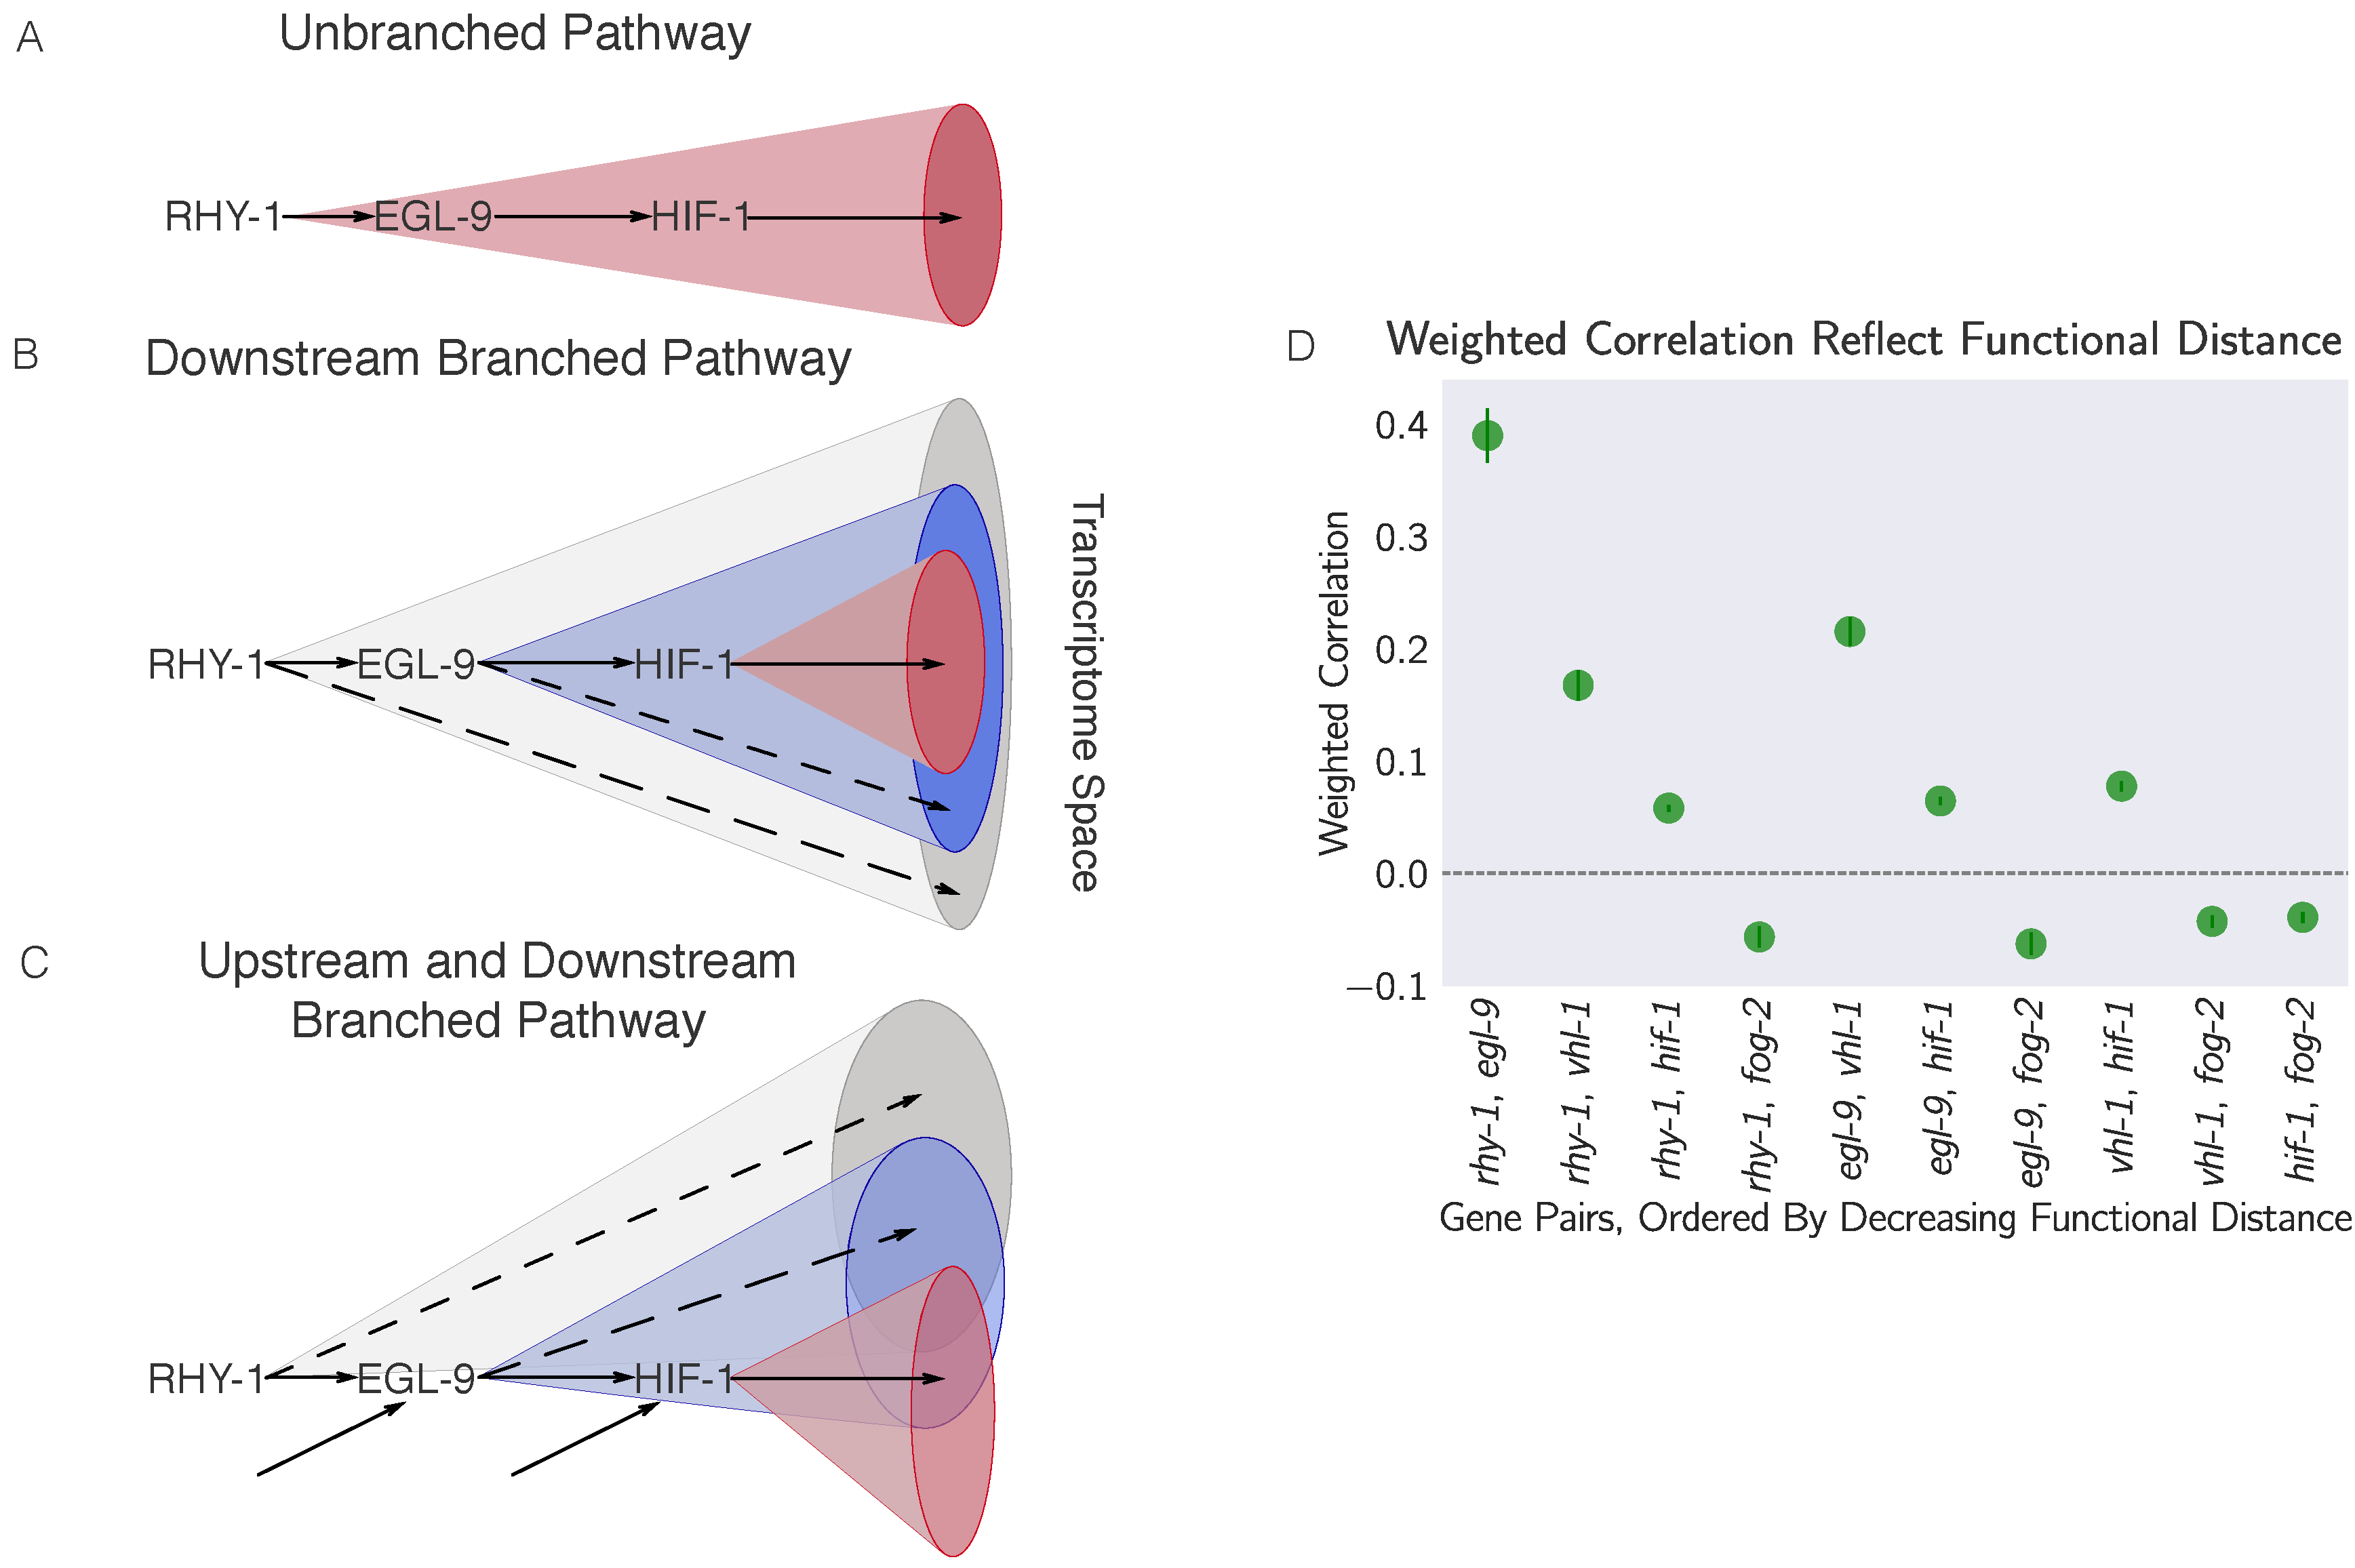
\includegraphics[width=.8\linewidth]{hypims/decorrelation-horizontal.pdf}
\caption{
Theoretically, transcriptomes can be used to order genes in a pathway under
certain assumptions. Arrows in the diagrams above are intended to show the
direction of flow, and do not indicate valence.
\textbf{A}. A linear pathway in which \gene{rhy-1} is the only gene controlling
\gene{egl-9}, which in turn controls \gene{hif-1} does not contain information
to infer the order between genes.
\textbf{B}. If \gene{rhy-1} and \gene{egl-9} have transcriptomic effects that are
separable from \gene{hif-1}, then the \gene{rhy-1} transcriptome should contain
contributions from \gene{egl-9}, \gene{hif-1} and \gene{egl-9}- and
\gene{hif-1}-independent pathways. This pathway contains enough information to
infer order.
\textbf{C}. If a pathway is branched both upstream and downstream,
transcriptomes will show even faster decorrelation. Nodes that are
separated by many edges may begin to behave almost independently of each other
with marginal transcriptomic overlap or correlation.
\textbf{D}. The hypoxia pathway can be ordered.
We hypothesize the rapid decay in correlation is due to a mixture of
upstream and downstream branching that happens along this pathway. Bars show the
standard error of the weighted coefficient from the Monte Carlo Markov Chain
computations.
}
\label{fig:decorrelation}
\end{figure}


We investigated the possibility that transcriptomic signals do in fact contain
relevant information about the degrees of separation by weighting the robust
Bayesian regression between each pair of genotypes by the size of the shared
transcriptomic phenotype of each pair divided by the total number of isoforms
differentially expressed in either mutant
($N_\mathrm{Intersection}/N_{\mathrm{Union}}$). We plotted the weighted
correlation of each gene pair, ordered by increasing functional distance
(see Fig.~\ref{fig:decorrelation}). In every case, we see that the weighted
correlation decreases monotonically due mainly, but not exclusively, to a smaller
STP.\@ We believe that this result is not due to random noise or insufficiently
deep sequencing. Instead, we propose a framework in which every gene is regulated
by multiple different molecular species, which induces progressive decorrelation.
This decorrelation in turn has two consequences. First, decorrelation within a
pathway implies that two nodes may be almost independent of each other if the
functional distance between them is large. Second, it may be possible to use
decorrelation dynamics to infer gene order in a branching pathway, as we have
done with the hypoxia pathway.

\subsection*{The circuit topology of the hypoxia pathway explains patterns in
            the data}
\label{sub:topology}
We noticed that while some of the rank plots contained a clear positive correlation
(see Fig.~\ref{fig:genetic_interactions}), other rank plots showed
a discernible cross-pattern (see Fig.~\ref{fig:xpattern}). In particular, this
cross-pattern emerged between \vhl{} and \rhy{} or between \vhl{} and \egl{},
even though genetically \gene{vhl-1}, \gene{rhy-1} and \gene{egl-9} are all
inhibitors of \hif{}. Such cross-patterns could be indicative of feedback loops
or other complex interaction patterns.

% correlative genetics again
\begin{figure}[tbhp]
\centering
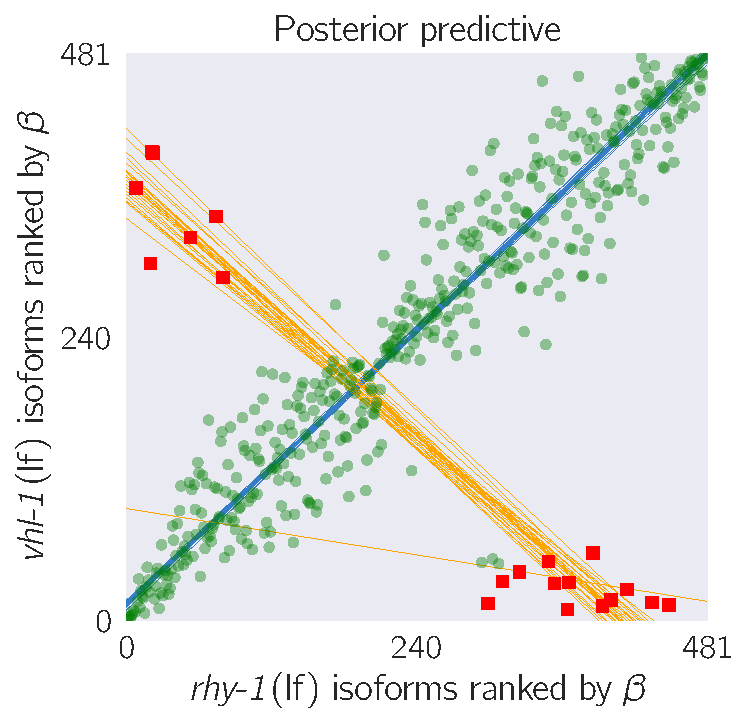
\includegraphics[width=.4\linewidth]{hypims/multiplemodes-ed.pdf}
\caption{
A feedback loop can generate transcriptomes that are both
correlated and anti-correlated. The \vhl{}/\rhy{} STP shows a cross-pattern.
Green large points are inliers to the first
regression. Red squares are outliers to the first regression. Only the red
small points were used for the secondary regression. Blue lines are representative
samples of the primary bootstrapped regression lines. Orange lines are
representative samples of the secondary bootstrapped regression lines.
}
\label{fig:xpattern}
\end{figure}



If the above is correct, then it should be possible to identify
\gene{egl-9}-independent, \rhy{}-dependent target genes in a
logically consistent way.
One erroneous way to identify these targets is via
subtractive logic. Using subtractive logic, we would identify genes that are
differentially expressed in \rhy{} mutants but not in \egl{} mutants.  Such a
gene set would
consist of almost 700 genes. One major drawback of subtractive logic is that it
cannot be applied when feedback loops exist between the genes in question.
Another problem is that the set of identified genes are statistically indistinguishable
from false positive and false negative hits because they have no distinguishing
property beyond the condition that they should be differentially expressed in
one mutant but not the other. In fact, this is exactly the behavior expected of
false-positive or false-negative hits---presence in one, but not multiple, mutants.
We need to consider the relationship between two genes before we can begin to
identify targets which expression is dependent on one gene and independent
of the other.

\gene{rhy-1} and \gene{egl-9} share a well-defined relationship. \rhyp{}
inhibits \cyslp{},
which in turn inhibits \eglp{}~\citep{Ma2012}. Therefore, loss of \rhyp{} leads
to inactivation of \eglp{}, which leads to increase in the cellular levels of
\hifp{}. \hifp{} in turn causes the mRNA levels of \gene{rhy-1} and \gene{egl-9}
to increase,
as they are involved in the \gene{hif-1}-dependent hypoxia response. However, since
\gene{rhy-1} has been mutated, the observed transcriptome is
\rhyp{} `null'; \eglp{} `null'; \hifp{} `on'. The situation is similar for
\egl{}, except that \rhyp{}
is not inactive, and therefore the observed transcriptome is the result of
\rhyp{} `up'; \eglp{} `null'; and \hifp{} `on'. From this pattern, we conclude that
the \egl{} and \rhy{} transcriptomes should exhibit a cross-pattern when plotted
against each other: The positive
arm of the cross is the result of the \eglp{} `null'; \hifp{} `on' dynamics; and the
negative arm reflects the different direction of \rhyp{} activity between
transcriptomes. No negative arm is visible (with the exception of two
outliers, which are annotated as pseudogenes in WormBase). Therefore, in this
dataset we do not find genes that have \gene{egl-9} independent,
\gene{rhy-1}-dependent expression patterns.

We also identified a main hypoxia response induced by disinhibiting
\gene{hif-1} (355 genes) by identifying genes that were commonly up-regulated
amongst \egl{}, \rhy{} and \vhl{} mutants. Although the hypoxic response is likely
to involve between three and seven times more genes (assuming the \rhy{} transcriptome
reflects the maximal hypoxic response), this is a conservative
estimate that minimizes false positive results, since these changes were
identified in four different genotypes with three replicates each. This response
included five transcription factors (\gene{W02D7.6}, \nhr{}, \gene{ztf-18},
\gene{nhr-135} and \gene{dmd-9}). The full list of genes associated with the
hypoxia response can be found in the Supplementary Table 1.
% TODO: SI numbering

\gene{hif-1}-independent effects of \gene{egl-9} have been reported
previously~\citep{Park2012}, which led us to question whether we could identify
similar effects in our dataset. We have observed that \hif{} displays a modest
increase in the transcription of \gene{rhy-1}, from which we speculated that
\eglp{} would have increased activity in the \hif{} mutant compared to the wild-type.
Therefore, we searched for genes that were regulated in an opposite manner between
\hif{} and \eglhif{}, and that were regulated in the same direction between
all \egl{} genotypes. We did not find any genes that met these conditions.

We also searched for genes with \gene{hif-1} independent, \gene{vhl-1}-dependent gene
expression and found \vhltargets{} genes, which can be found in the Supplementary
Table 2.
Finally, we searched for candidates directly regulated by \gene{hif-1}. Initially, we
searched for genes that had were significantly altered in \hif{} genotypes in one
direction, but altered in the opposite direction in mutants that activate the
\hifp{} response. Only two genes (\emph{R08E5.3}, and \emph{nit-1}) met these
conditions. This could reflect the fact that \hifp{} exists at very low
levels in \cel{}, so loss of function mutations in \gene{hif-1} might only have
mild effects on its transcriptional targets. We reasoned that genes
that are overexpressed in mutants that induce the \hifp{} response would be enriched
for genes that are direct candidates.  We found \hiftargets{}  genes which have
consistently increased expression in mutants with a constitutive hypoxic response.
These genes can be found in the Supplementary Table 3.


\subsubsection*{Enrichment analysis of the hypoxia response}
\label{sub:ea_hypoxia}
To validate that our transcriptomes were correct, and to understand how
functionalities may vary between them, we subjected each decoupled response to
enrichment analysis using the WormBase Enrichment Suite~\citep{Angeles-Albores2016,
Angeles-Albores2016b}.

\begin{figure}[tbhp]
\centering
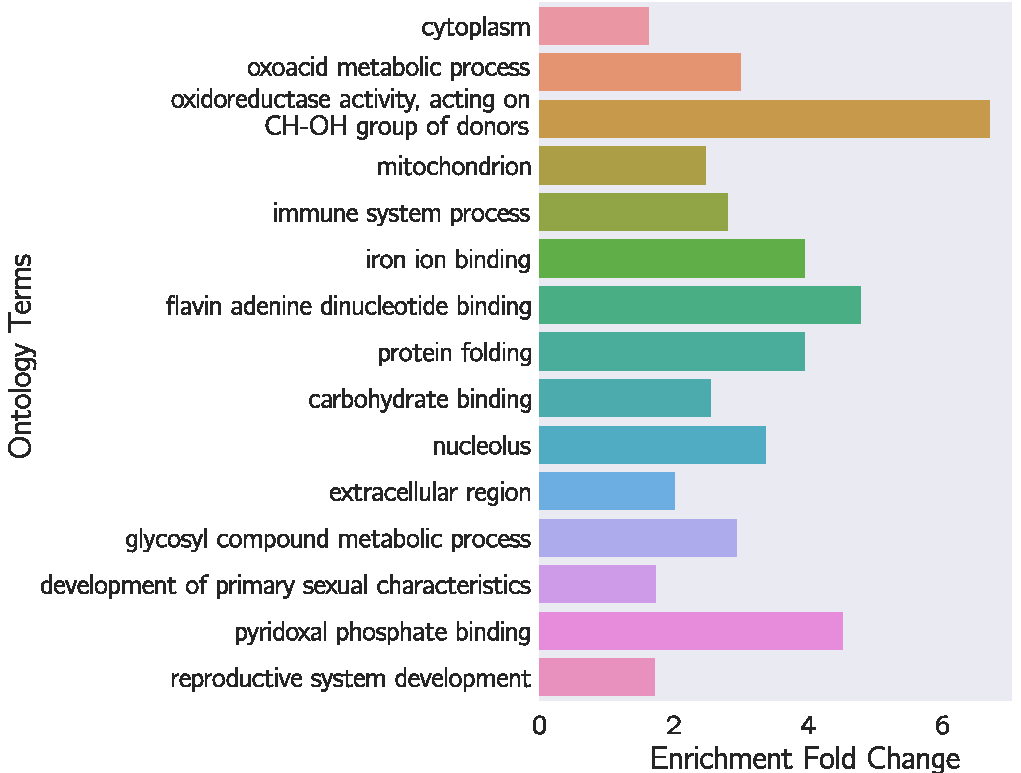
\includegraphics[width=.5\linewidth]{hypims/hypoxia_response_gea.pdf}
\caption{
Gene ontology enrichment analysis of genes associated with the main hypoxia response.
A number of terms reflecting catabolism and bioenergetics are enriched.
}
\label{fig:hyp_gea}
\end{figure}

We used gene ontology enrichment analysis (GEA) on the main hypoxia response program.
This showed that the terms `oxoacid metabolic process' (\qval{4}, 3.0 fold-change,
24 genes), `iron ion binding' (\qval{2}, 3.8 fold-change, 10 genes), and `immune
system process' (\qval{3}, 2.9 fold-change, 20 genes) were significantly enriched.
GEA also showed enrichment of the term `mitochondrion' (\qval{3}, 2.5 fold-change,
29 genes) (see Fig.~\ref{fig:hyp_gea}). Indeed, \hif{} has been implicated in
all of these biological and molecular functions~\citep{Luhachack2012,Ackerman2012,
Romney2011,Semenza2011}.
As benchmark on the quality of our data, we selected a set of 22 genes known to
be responsive to \hifp{} levels from the literature and asked whether these genes
were present in our hypoxia response list. We found $8/22$ known genes, which
constitutes a statistically significant result ($p<10^{10}$). The small number of
reporters found in this list probably reflects the conservative nature of our
estimates.
We studied the \gene{hif-1}-independent, \gene{vhl-1}-dependent gene set
using enrichment analysis but no terms were significantly enriched.

\subsection*{Identification of non-classical epistatic interactions}
\label{sub:hifoh}
\hif{} has traditionally been viewed as existing in a genetic OFF state under
normoxic conditions. However, our dataset indicates that \hifn{} genes show
altered expression when \gene{hif-1} function is removed in normoxic conditions.
Moreover, we observed positive correlations between \hif{} $\beta$ coefficients
and \egl{}, \vhl{} and \rhy{} $\beta$ coefficients in spite of the negative
regulatory relationships between these genes and \gene{hif-1}. Such
positive correlations could indicate a different relationship between these genes
than has previously been reported, so we attempted to substantiate them through
epistasis analyses.

To perform epistasis analyses, we first identified genes that exhibited violations
of the canonical genetic model of the hypoxia pathway. To this end, we searched for
genes that exhibited different behaviors between \egl{} and \vhl{}, or
between \rhy{} and \vhl{} (we assume that all results from the
\rhy{} transcriptome reflect a complete loss of \gene{egl-9} activity). We found
\hifohtargets{} that satisfied this condition (see Fig.~\ref{fig:hif1oh},
Supplemental Table 4).
Additionally, many of these genes exhibited a new kind of epistasis. Namely,
\gene{egl-9} was epistatic over \gene{vhl-1}. Identification of a set of genes
that have a consistent set of relationships between themselves suggests that
we have identified a new aspect of the hypoxia pathway.

\begin{figure}[tbhp]
\centering
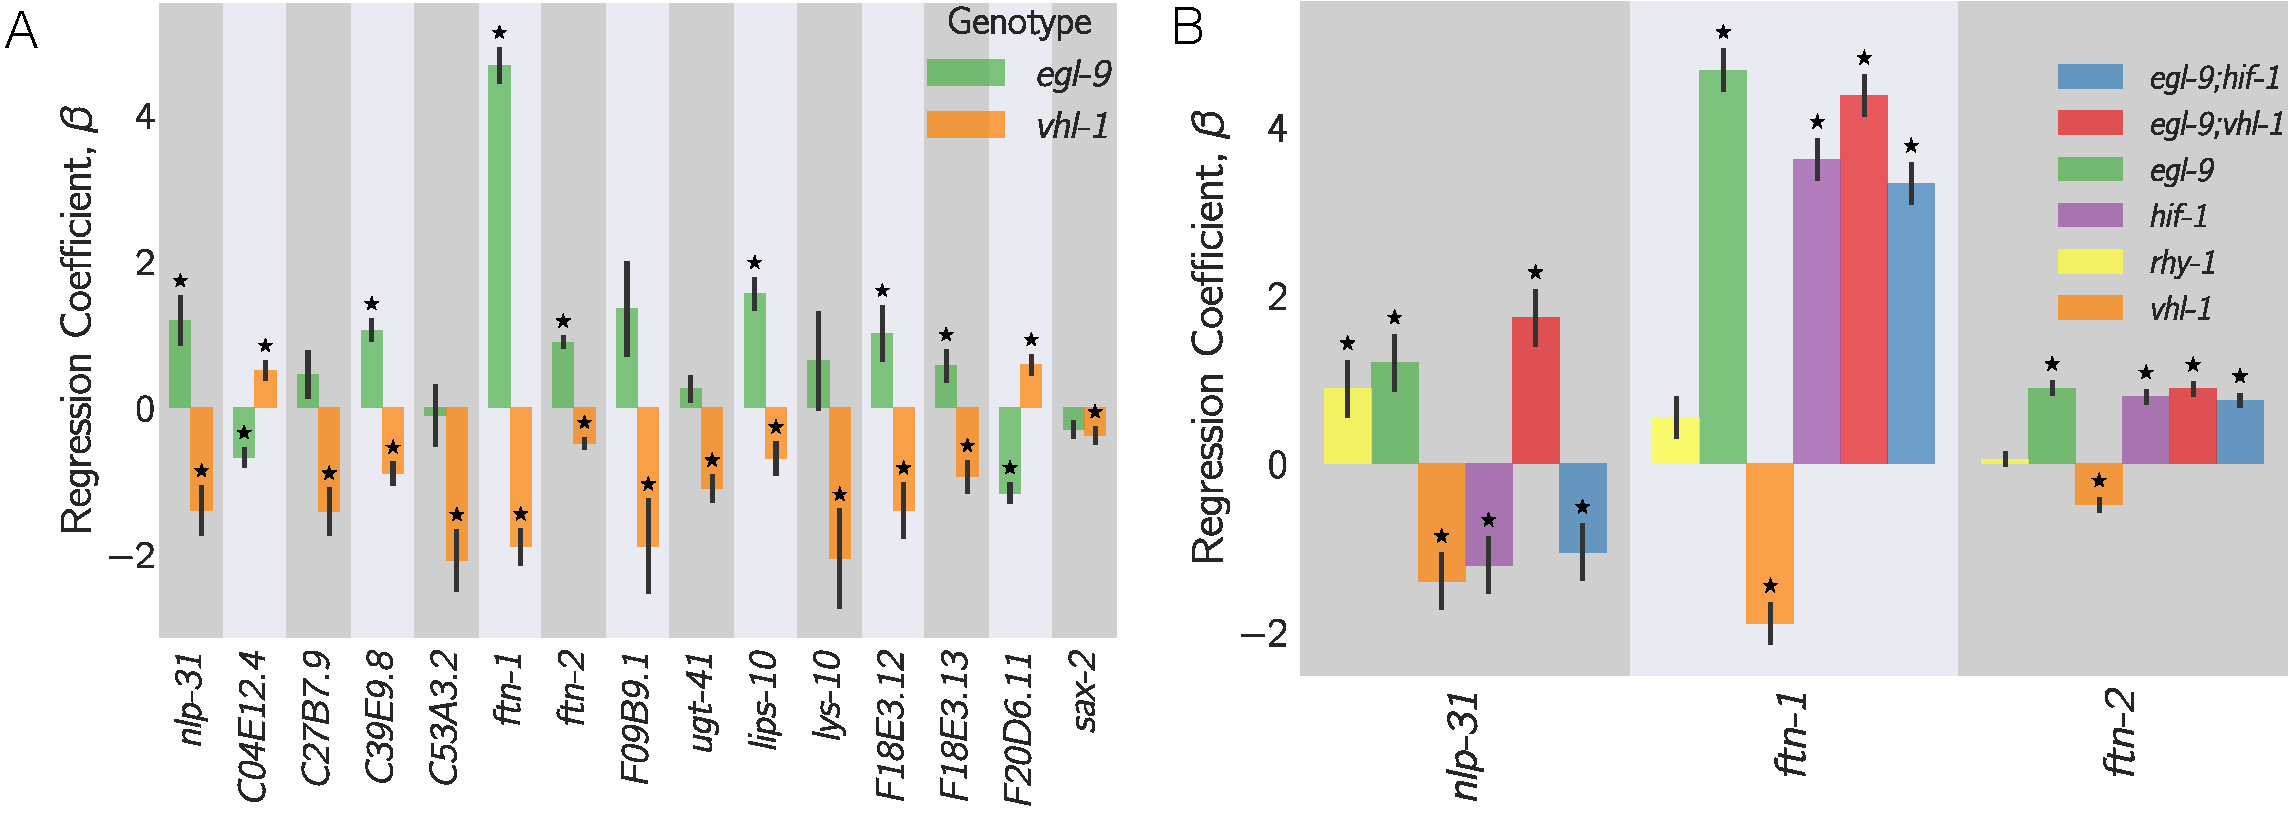
\includegraphics[width=.9\linewidth]{hypims/hif1oh-epistasis-horizontal.pdf}
\caption{
\textbf{A}. 27 genes in \cel{} exhibit non-classical epistasis in the hypoxia
pathway, characterized by opposite effects on gene expression, relative to the
wild-type, of of the \vhl{} compared to \egl{} (or
\rhy{}) mutants. Shown are a random selection of 15 the 27 genes for illustrative
purposes.
\textbf{B}. Representative genes showing that non-canonical epistasis shows a
consistent pattern. \vhl{} mutants have an opposite effect to \egl{}, but
\gene{egl-9} remains epistatic to \gene{vhl-1} and loss-of-function mutations in
\gene{hif-1} suppress the \egl{} phenotype. Asterisks show $\beta$ values
significantly different from 0 relative to wild-type (\qval{1}).
}
\label{fig:hif1oh}
\end{figure}

To illustrate this, we focused on three genes, \nlp{}, \ftna{} and \ftnb{}, which
epistasis patterns that we felt reflected the population well. \ftna{} and \ftnb{}
are both described in the literature as genes that are responsive to mutations in
the hypoxia pathway. Moreover, these genes have been previously described to have
aberrant behaviors~\citep{Ackerman2012,Romney2011}, specifically the
opposite effects of \egl{} and \vhl{}. These studies showed that loss of \vhl{}
decreases expression of \ftna{} and \ftnb{} using both RNAi and alleles, which
allays concerns of strain-specific interference. Moreover, Ackerman and Gems (2012)
showed that \gene{vhl-1} is epistatic to \gene{hif-1} for the \ftna{}
expression phenotype, and that loss of
\hifp{} is associated with increased expression of \ftna{} and \ftnb{}. We observed
that \gene{hif-1} was epistatic to \gene{egl-9}, and that \gene{egl-9} and
\gene{hif-1} both promoted \ftna{} and \ftnb{} expression.

Epistasis analysis of \ftna{} and \ftnb{} expression reveals that \gene{egl-9} is
epistatic to \gene{hif-1}; that \gene{vhl-1} has opposite effects to \gene{egl-9},
and that \gene{vhl-1} is epistatic to \gene{egl-9}. Analysis of \nlp{}
reveals similar relationships. \nlp{} expression is decreased in \hif{},
and increased in \egl{}. However, \gene{egl-9} is epistatic to \gene{hif-1}.
Like \ftna{} and \ftnb{}, \gene{vhl-1} has the opposite effect to \gene{egl-9},
yet is epistatic to \gene{egl-9}. We propose in the Discussion a model for how
\hifp{} might regulate these targets.

\subsection*{\hifp{} in the cellular context}
\label{sub:metabolism}

We identified the transcriptional changes
associated with bioenergetic pathways in \cel{} by extracting from
WormBase all genes associated with the tricarboxylic acid (TCA) cycle, the
electron transport chain (ETC) and with the \cel{} GO term energy reserve.
Previous research has described the effects of mitochondrial dysfunction in
eliciting the hypoxia response~\citep{Lee2010}, but transcriptional feedback
from \hifp{} into bioenergetic pathways has not been as extensively in \cel{},
as in vertebrates (see, for example~\citep{Semenza1994,Semenza2012}).
We also searched for the changes in ribosomal components and the proteasome, as
well as for terms relating to immune response (see Fig~\ref{fig:genomewide}).

\begin{figure}[tbhp]
\centering
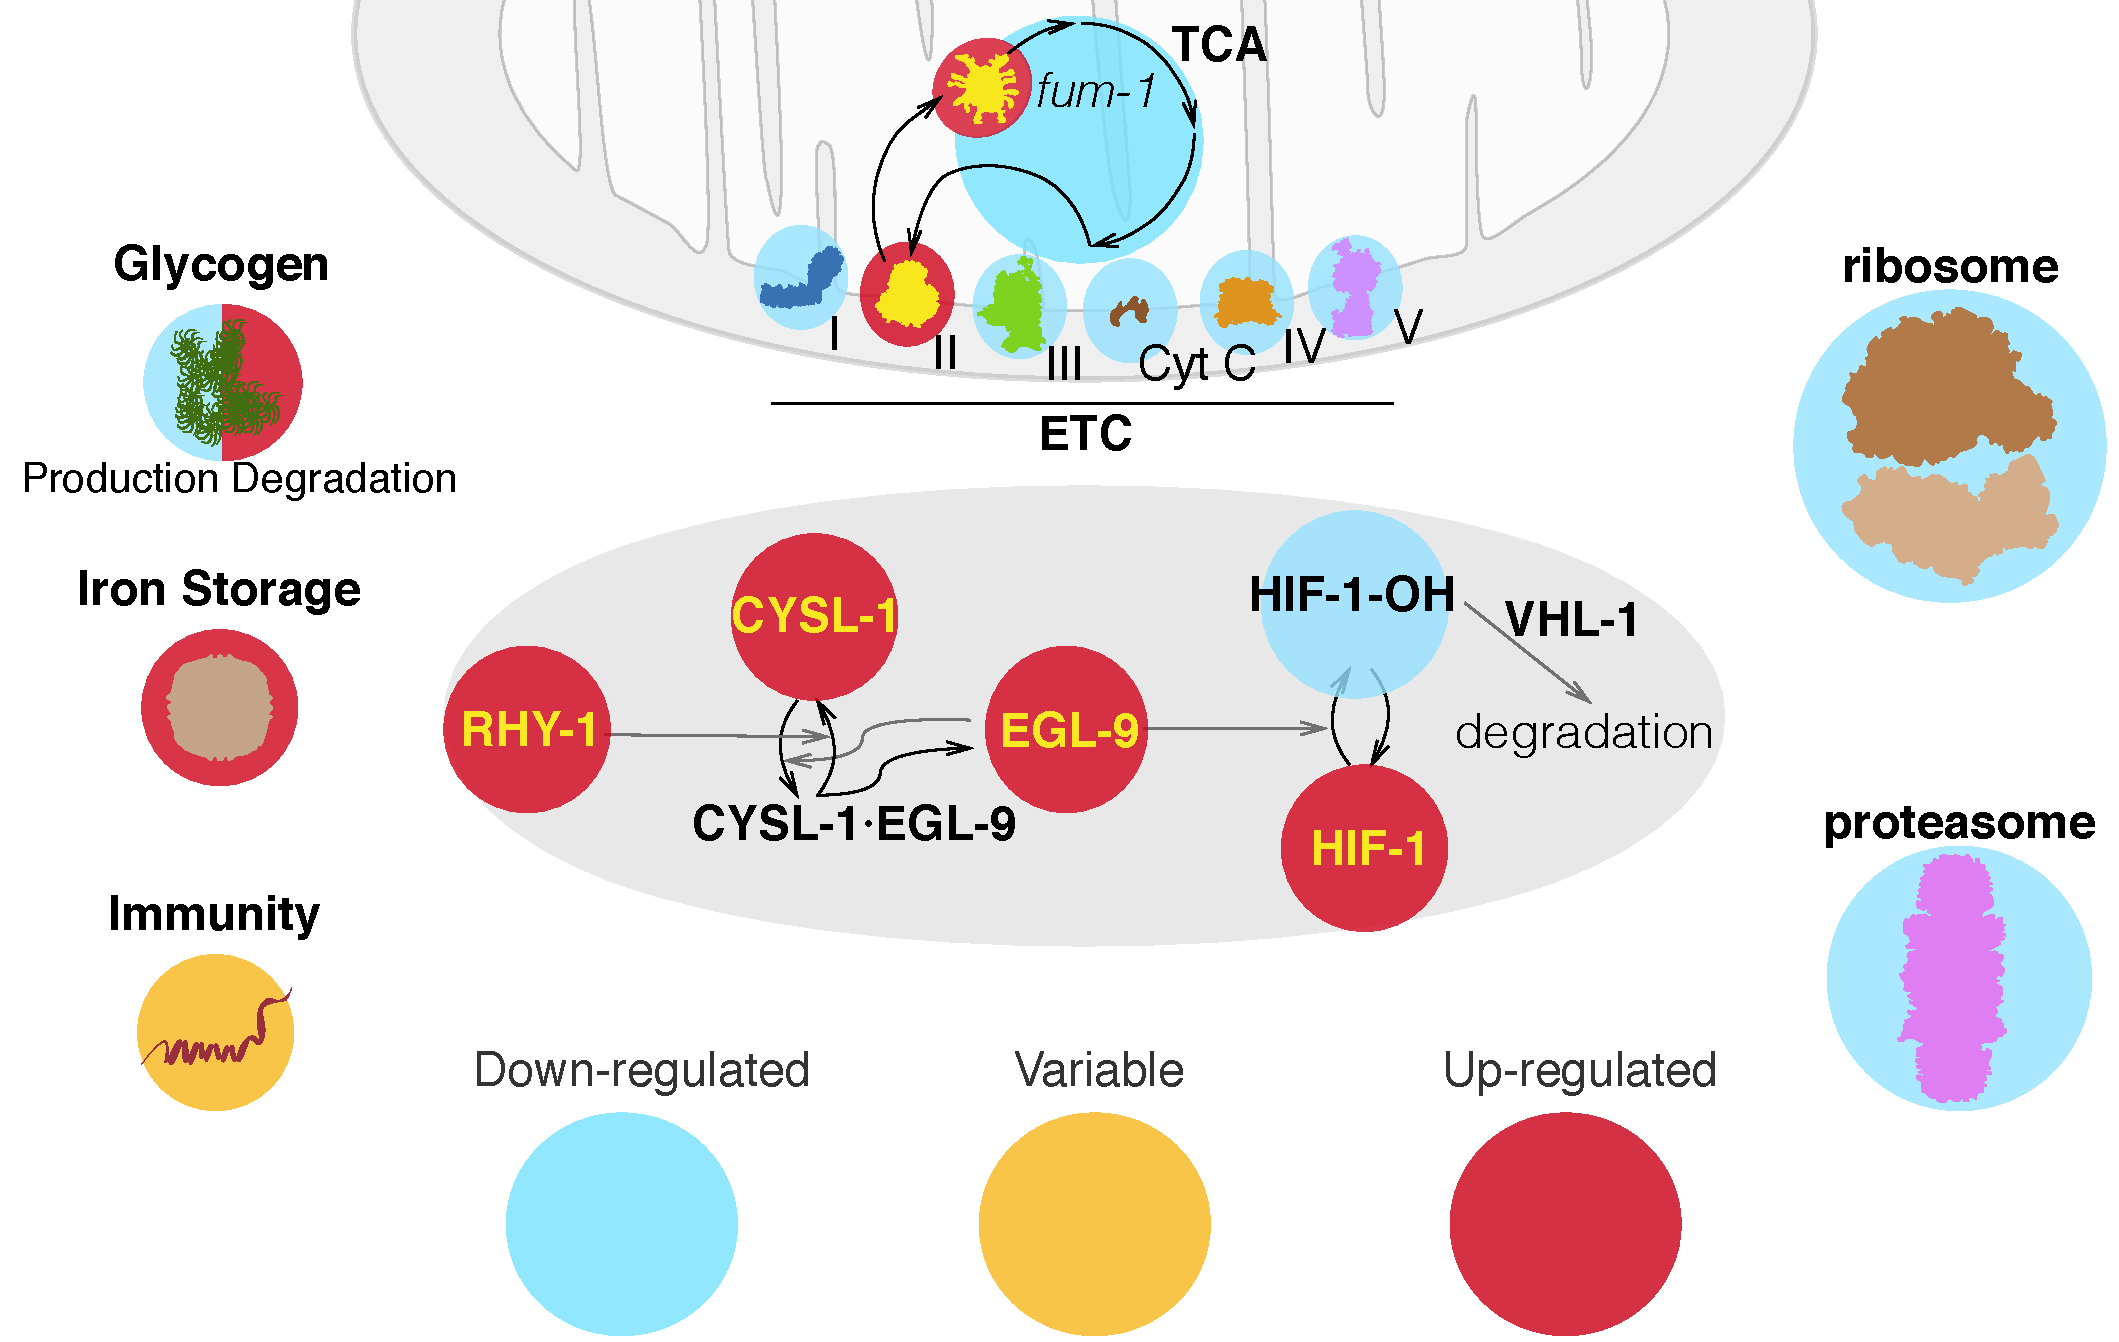
\includegraphics[width=.7\linewidth]{hypims/hif1genomewide.pdf}
\caption{
A graphic summary of the genome-wide effects of \hifp{} from our RNA-seq data.
}
\label{fig:genomewide}
\end{figure}

\subsubsection*{Bioenergetic pathways}
Our data shows that most of the enzymes involved in the TCA cycle and in the ETC
are down-regulated when \hifp{} is induced in agreement with the previous
literature~\citep{Semenza2012}.
However, the fumarase gene \gene{fum-1} and the mitochondrial complex II stood out
as notable exceptions to the trend, as they were up-regulated in every single
genotype that causes deployment of the hypoxia response. FUM-1 catalyzes the
reaction of fumarate into malate, and complex II catalyzes the reaction of
succinate into fumarate. Complex II has been identified as a source of reserve
respiratory capacity in neonatal rat cardiomyocytes previously~\citep{Pfleger2015}.
We found two energy reserve genes that were down-regulated by \hifp{}.
\gene{aagr-1} and \gene{aagr-2}, which are predicted to function in glycogen
catabolism~\citep{Sikora2010}.
Three distinct genes involved in energy reserve were up-regulated. These genes were
\gene{ogt-1}, which encodes O-linked GlcNac Transferase gene; \gene{T04A8.7},
encoding an ortholog of human glucosidase, acid beta (GBA); and \gene{T22F3.3},
encoding ortholog of human glycogen phosphorylase isozyme in the muscle (PYGM).

\subsubsection*{Protein synthesis and degradation}
\hif{} is also known to inhibit protein synthesis and translation in varied
ways.~\citep{Brugarolas2004}. Most reported effects of
\hifp{} on the translation machinery are posttranslational, and no reports to date
show transcriptional control of the ribosomal machinery in \cel{} by \hifp{}. We
used the WormBase Enrichment Suite Gene Ontology
dictionary~\citep{Angeles-Albores2016b} to extract 143 protein-coding genes
annotated as `structural constituents of the ribosome' and we queried whether
they were differentially expressed in our mutants. \egl{}, \vhl{}, \rhy{} and
\egl{};\vhl{} showed differential expression of 91 distinct ribosomal constituents
(not all constituents were detected in all genotypes). For every one of these
genotypes, these genes were always down-regulated. In contrast, \hif{} showed
up-regulation of a single ribosomal constituent.

Next, we asked whether \hifp{} has any transcriptional effects on the
proteasomal constituents; no such effects of \hifp{} on the proteasome
have been reported in \cel{}. Out of 40 WormBase-annotated proteasomal constituents,
we found 31 constituents that were differentially expressed in at least one of the
four genotypes that induce a hypoxic response. Every gene we found was down-regulated
in at least two out of the four genotypes we studied.

\section*{Discussion}
\subsection*{The \cel{} hypoxia pathway can be reconstructed entirely from
             RNA-seq data}
In this paper, we have shown that whole-organism transcriptomic phenotypes
can be used to reconstruct genetic pathways and to discern previously overlooked
or uncharacterized genetic interactions. We successfully reconstructed the hypoxia
pathway, and inferred order of action (\gene{rhy-1} activates \gene{egl-9},
\gene{egl-9} and \gene{vhl-1} inhibit \gene{hif-1}), and we were able to infer
from transcriptome-wide epistasis measurements that \gene{egl-9} exerts
\gene{vhl-1}-dependent and independent inhibition on \gene{hif-1}.

\subsection*{\hifp{} and the cellular environment}

In addition to reconstructing the pathway, our dataset allowed us
to observe a wide variety of physiologic changes that occur as a result of the
\hifp{}-dependent hypoxia response. In particular, we observed down-regulation of most
components of the TCA cycle and the mitochondrial electron transport chain with
the exceptions of \gene{fum-1} and the mitochondrial complex II.\@ The mitochondrial
complex II catalyzes the reaction of succinate into fumarate.
In mouse embryonic fibroblasts, fumarate has been
shown to antagonize \hifp{} prolyl hydroxylase domain (PHD) enzymes, which are
orthologs of \eglp{}~\citep{Sudarshan2009}.
If the inhibitory role of fumarate on PHD enzymes is conserved in \cel{},
upregulation of complex II by \hifp{} during hypoxia may increase
intracellular levels of fumarate, which in turn could lead to artificially high
levels of \hifp{}
even after normoxia resumes. The increase in fumarate produced by the complex
could be compensated by increasing expression of \gene{fum-1}. Increased fumarate
degradation allows \cel{} to maintain plasticity in the hypoxia pathway, keeping
the pathway sensitive to oxygen levels.

\subsection*{Interpretation of the non-classical epistasis in the hypoxia pathway}
The observation of almost 30 genes that exhibit a specific pattern of non-classical
epistasis suggests the existence of previously undescribed aspects of the hypoxia
pathway. Some of these non-classical epistases had been observed
previously~\citep{Ackerman2012,Romney2011,Luhachack2012}, but
no satisfactory mechanism has been proposed to explain this biology.
\citet{Romney2011} and \citet{Ackerman2012}
suggest that \hifp{} integrates information on iron concentration in the
cell to bind to the \ftna{} promoter, but could not definitively establish
a mechanism.
It is unclear why deletion of \gene{hif-1} induces \ftna{}
expression, deletion of \gene{egl-9} also causes induction of \ftna{} expression,
but deletion of \gene{vhl-1} removes this inhibition. Moreover, \citet{Luhachack2012}
have previously reported that certain genes important for the \cel{} immune response
against pathogens reflect similar expression patterns. Their interpretation
was that \gene{swan-1}, which encodes a binding partner to \eglp{}~\citep{Shao2010},
is important for modulating \hifp{} activity in some manner. The lack of a
conclusive double mutant analysis in this work means the role of SWAN-1 in
modulation of \hifp{} activity remains to be demonstrated. Nevertheless, mechanisms
that call for additional transcriptional modulators become less likely given the
number of genes with different biological functions that exhibit the same pattern.

\begin{figure}[tbhp]
\centering
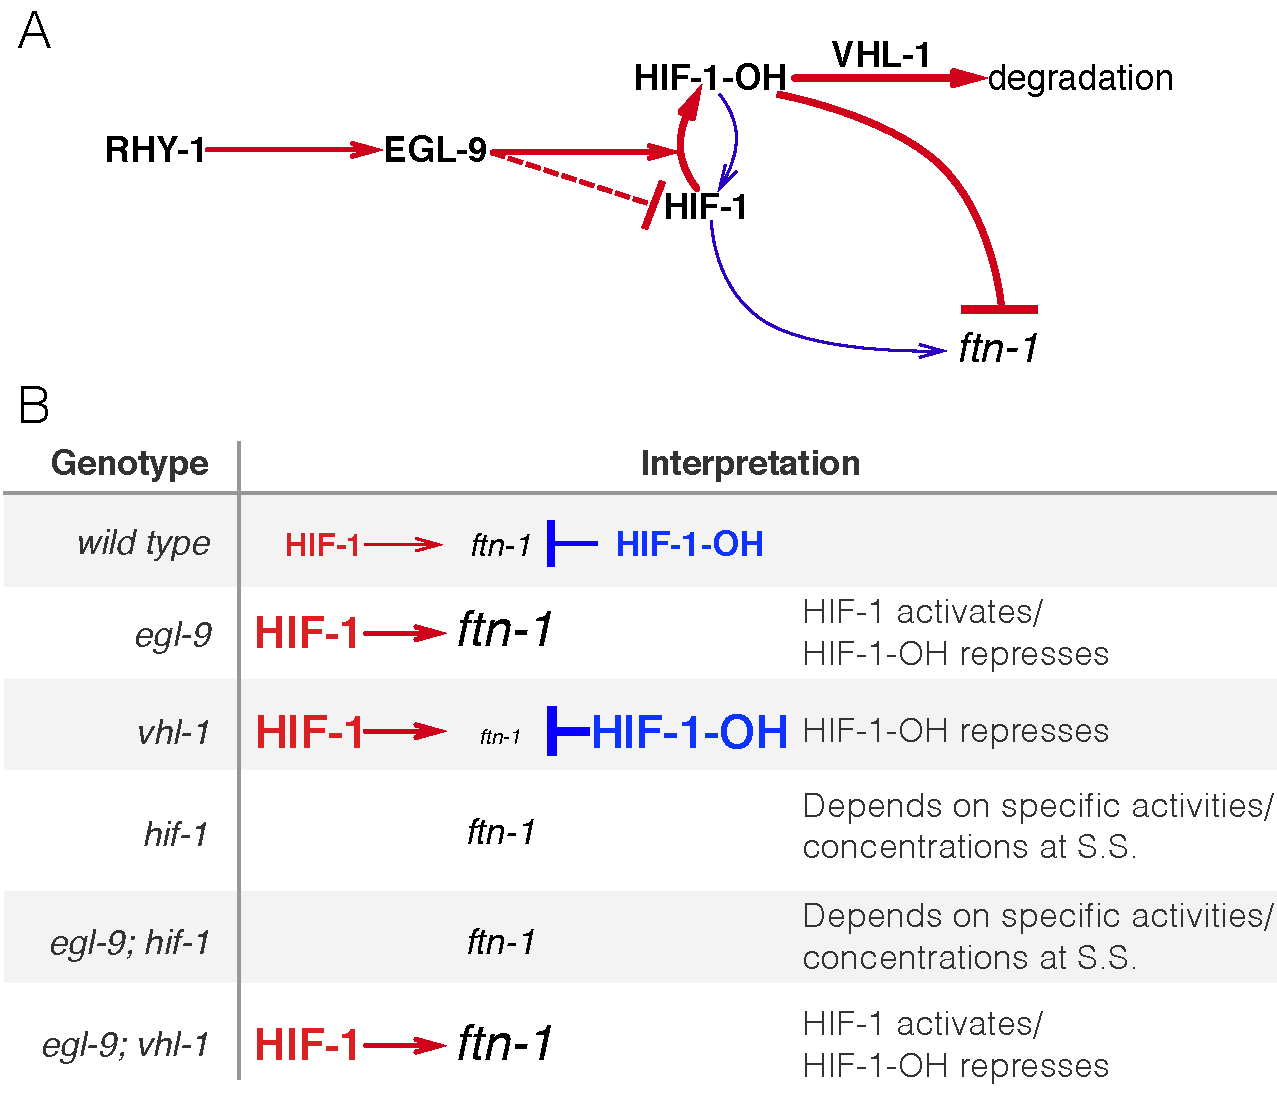
\includegraphics[width=.5\linewidth]{hypims/hif1oh_model.pdf}
\caption{
A hypothetical model showing a mechanism where \hifp{}-hydroxyl antagonises
\hifp{}.
\textbf{A}. Diagram showing that RHY-1 activates EGL-9.
EGL-9 hydroxylates HIF-1 in an oxygen dependent fashion. Under normoxia, HIF-1
is rapidly hydroxylated and only slowly does hydroxylated HIF-1 return to its
original state. EGL-9 can also inhibit HIF-1 in an oxygen-independent fashion.
HIF-1 hydroxyl is rapidly degraded in a VHL-1 dependent fashion. In our model,
HIF-1 and HIF-1 hydroxyl have opposing effects on transcription. The width of the
arrows represents the rates under normoxic conditions.
\textbf{B}. Table showing the effects of loss-of-function mutations on HIF-1 and
HIF-1 hydroxyl activity, showing how this can potentially explain the behavior
of \gene{ftn-1} in each case.  S.S = Steady-state.
}
\label{fig:hif1oh_table}
\end{figure}

One way to resolve this problem without invoking additional genes is to
consider \hifp{} as a protein with both activating and inhibiting states. In fact,
\hifp{} already exists in two states in \cel{}: unmodified \hifp{} and
\hifp{}-hydroxyl (\hifp{}-OH). Under this model, \hifp{}-hydroxyl antagonizes
the effects of \hifp{} for certain genes like \ftna{} or \nlp{}. Loss of
\gene{vhl-1} stabilizes \hifp{}-hydroxyl.
A subset of genes that are sensitive to \hifp{}-hydroxyl will be inhibited as a
result of the increase in the amount of this species, in spite of loss of
\gene{vhl-1} function also increasing the level of non-hydroxylated \hifp{}.
On the other hand, \egl{} selectively removes all \hifp{}-hydroxyl, stimulating
accumulation of \hifp{} and promoting gene activity. Whether deletion of \hif{}
is overall activating or inhibiting will depend on the relative activity of each
protein state under normoxia (see Fig.~\ref{fig:hif1oh_table}).

Multiple lines of circumstantial evidence that \hifp{}-hydroxyl plays a role
in the functionality of the hypoxia pathway. First, \hifp{}-hydroxyl is
challenging to study genetically because no mimetic mutations are available with
which to study the pure hydroxylated \hifp{} species. Second, although mutations in
the Von-Hippel Landau gene stabilize the hydroxyl species, they also increase the
quantity of non-hydroxylated \hifp{} by mass action.
Finally, since \hifp{} is detected low levels
in cells under normoxic conditions~\citep{Wang1993}, total \hifp{} protein
(unmodified \hifp{} plus \hifp{}-hydroxyl) is often tacitly assumed to be
vanishingly rare and therefore biologically inactive.

Our data show hundreds of genes that change expression in response
to loss of \gene{hif-1} under normoxic conditions. This establishes that there is
sufficient total \hifp{} protein to be biologically active.
Our analyses also revealed that \hif{} shares
positive correlations with \egl{}, \rhy{} and \vhl{}, and that each of these genotypes
also shows a secondary negative rank-ordered expression correlation with each other.
These cross-patterns between all loss of function of inhibitors of \hifp{} and
\hif{} can be most easily explained if \hifp{}-hydroxyl is biologically active.

A homeostatic argument can be made in favor of the activity of \hifp{}-hydroxyl.
At any point in time, the cell must measure the levels of
multiple metabolites at once. The \gene{hif-1}-dependent hypoxia
response integrates information from O$_2$, $\alpha$-ketoglutarate
(2-oxoglutarate) and iron concentrations in the cell. One way to
integrate this information is by encoding it only in the effective hydroxylation
rate of \hifp{} by \eglp{}. Then the dynamics in this system will evolve
exclusively as a result of the total amount of \hifp{} in the cell. Such a system
can be sensitive to fluctuations in the absolute concentration of
\hifp{}~\citep{Goentoro2009a}. Since the absolute levels of \hifp{} are low in
normoxic conditions, small fluctuations in protein copy-number represent can
represent a large fold-change in \hifp{} levels. These fluctuations would
not be problematic for genes that must be turned on only under conditions of severe
hypoxia---presumably, these genes would be associated with low affinity
sites for \hifp{}, so that they are only activated when \hifp{} levels are far
above random fluctuations.

For yet other sets of genes that must change expression in response to the hypoxia
pathway, it may not make as much sense to integrate metabolite information
exclusively via \eglp{}-dependent hydroxylation of \hifp{}. In particular, genes
that may function to increase survival in mild hypoxia may benefit from regulatory
mechanisms that can sense minor changes in environmental conditions and which
therefore benefit from robustness to transient changes in protein copy number.
Likewise, genes that are involved in iron or $\alpha$-ketoglutarate metabolism
(such as \ftna{}) may benefit from being able to sense, accurately, small and
consistent deviations from basal concentrations of these metabolites. For these
genes, the information may be better encoded by using \hifp{} and
\hifp{}-hydroxyl as an activator/repressor pair. Such circuits are
known to possess distinct advantages for controlling output in a manner that
is robust to transient fluctuations in the levels of their
components~\citep{Hart2012,Hart2013}.

Our RNA-seq data suggests that one of these atypical targets of \hifp{}
may be \rhyp{}. Although \gene{rhy-1} does not exhibit non-classical
epistasis, \hif{} and \eglhif{} both had increased expression levels of \gene{rhy-1}.
We speculate that if \gene{rhy-1} is controlled by both \hifp{} and \hifp{}-hydroxyl,
then this might imply that \hifp{} regulates the expression of its pathway (and
therefore itself) in a manner that is robust to total \hifp{} levels.

\subsection*{Insights into genetic interactions from vectorial phenotypes}

Here, we have described a set of straightforward methods that can be in theory
applied to any vectorial phenotype. Genome-wide methods afford a lot of information,
but genome-wide interpretation of the results is often extremely challenging.
Each method has its own advantages and disadvantages. We briefly discuss these
methods, their uses and their drawbacks.

Principal component analysis
is computationally tractable and clusters can often be visually detected with
ease. However, PCA can be misleading, especially when the dimensions represented
do not explain a very large fraction of the variance present in the data. In addition,
principal dimensions are the product of a linear combination of vectors, and therefore
must be interpreted with extreme care. In this case, the first principal dimension
separated genotypes that increase \hifp{} protein levels from those that decrease
it, but this dimension is a mix of vectors of change in gene expression. Although
PCA showed that there is information hidden in these genotypes, it was not enough
by itself to provide biological insight.

Whereas PCA operates on all genotypes simultaneously, correlation analysis is a
pairwise procedure that measures how predictable the gene
expression changes are in a mutant given the vector of expression changes in
another. Like PCA, correlation analysis is easy and fast to perform. Unlike PCA,
the product of a correlation analysis is a single number with a straightforward
interpretation. However, correlation analysis is particularly sensitive to outliers.
Although a common strategy is to rank-transform expression data to mitigate
outliers, rank-transformations do not remove the cross-patterns that appear when
feedback loops or other complex interactions are present between two genes.
Such cross-patterns can still lead to vanishing correlations if both patterns are
equally strong. Therefore, correlation analyses must take into account the possible
existence of systematic outliers. Moreover, correlation values must be measured
for both interactions in cross-patterned rank plots. Weighted correlations could
be informative for ordering genes along pathways.
A drawback of correlation
analysis is that the number of pairwise comparisons that must be made increases
combinatorially, though strategies could be used to decrease the total number of
effective comparisons.

Epistasis plots are a novel way to visualize epistasis in vectorial phenotypes.
Here, we have shown how an epistasis plot can be used to identify interactions
between two single mutants and a double mutant. In reality, epistasis plots
can be generated for any set of measurements involving a set of $N$ mutants and
an $N$-mutant genotype. Epistasis plots can accumulate an arbitrary number of
points within them, possess a rich structure that can be visualized and have
straightforward interpretations for special slope values.

Another way to analyze epistasis is via general linear models (GLMs) that include
interaction terms between two or more genes. In this way, GLMs can quantify
the epistatic effect of an interaction on single genes. We and
others~\citep{Dixit2016,Angeles-Albores2016a} have previously used GLMs to identify
gene sets that are epistatically regulated by two or more inputs. While powerful,
GLMs suffer from the multiple comparison problem. Correcting for false positives
using well-known multiple comparison corrections such as FDR~\citep{Storey2003}
tends to increase false negative rates.  Moreover, since GLMs attempt to estimate
effect magnitudes for individual gene or isoform expression levels, they
effectively treat each gene as an independent quantity, which prevents better
estimation of the magnitude and direction of the epistasis between two genes.

Epistasis plots do not suffer from the multiple comparison problem because the
number of tests performed is orders of magnitudes smaller than the number
of tests performed by GLMs. Ideally, in an epistasis plot we need only perform
3 tests---rejection of additive, unbranched and suppressive null models---compared
with the tens of thousands of tests that are performed in GLMs. Moreover, the
magnitude of epistasis between two genes can be estimated using hundreds of genes,
which greatly improves the statistical resolution of the epistatic coefficient.
This increased resolution is important because the size and magnitude of the
epistasis has specific consequences for the type of pathway that is expected.

Any quantitative use of genome-wide datasets requires a good experimental setup.
Here, we have demonstrated that whole-organism RNA-seq can be used to dissect
molecular pathways in exquisite detail when paired with experimental designs that
are motivated by classical genetics. Much more research will be necessary
to understand whether epistasis has different consequences in the microscopic
realm of transcriptional phenotypes than in the macroscopic world that geneticists
have explored previously. Our hope is that these tools, coupled with the classic
genetics experimental  designs, will reveal hitherto unknown aspects of genetics
theory.

\section*{Methods}
\label{sec:methods}
\subsection*{Nematode strains and culture}
Strains used were N2 wild-type Bristol,
CB5602 \gene{vhl-1}(\emph{ok161}),
CB6088 \gene{egl-9}(\emph{sa307})~\gene{hif-1}(\emph{ia4}),
CB6116 \gene{egl-9}(\emph{sa307});\gene{vhl-1}(\emph{ok161}),
JT307 \gene{egl-9}(\emph{sa307}),
ZG31 \gene{hif-1}(\emph{ia4}),
RB1297 \gene{rhy-1}(\emph{ok1402}).
All lines were grown on standard
nematode growth media (NGM) plates seeded with OP50 \ecol{} at 20\degree{}C
(Brenner 1974).

\subsection*{RNA Isolation}
Unsynchronized lines were grown on NGM plates at 20C and eggs harvested by
sodium hypochlorite treatment. Eggs were plated on 6 to 9 6cm NGM plates
with ample OP50 \ecol{} to avoid starvation and grown at
20\degree{}C.  Worms were staged and harvested based on the time after plating,
vulva morphology and the absence of eggs.  Approximately 30--50 non-gravid young
adults were picked and placed in 100$\mu$L of TE pH 8.0 at 4\degree{}C in
$0.2$mL PCR tubes.   After settling and a brief spin in microcentrifuge
approximately $80\mu$L of TE (Ambion AM 9849) was removed from the top of the
sample and individual replicates
were snap frozen in liquid N2. These replicate samples were then digested with
Proteinase K (Roche Lot No. 03115 838001 Recombinant Proteinase K PCR Grade) for
15min at 60\degree{} in the presence of 1\% SDS and 1.25$\mu$L
RNA Secure (Ambion AM 7005). RNA samples were then taken up in 5 Volumes of
Trizol (Tri Reagent Zymo Research) and processed and treated with DNase I using
Zymo MicroPrep RNA Kit (Zymo Research Quick-RNA MicroPrep R1050).
RNA was eluted in RNase-free water and divided into aliquots and stored at
-80\degree{}C. One aliquot of each replicate was analyzed using a NanoDrop (Thermo
Fisher) for impurities, Qubit for concentration and then analyzed on an Agilent
2100 BioAnalyzer (Agilent Technologies).
Replicates were selected that had RNA integrity numbers (RIN) equal or greater
than 9.0 and showed no evidence of bacterial ribosomal bands, except for the
ZG31 mutant where one of three replicates had a RIN of 8.3.

\subsection*{Library Preparation and Sequencing}
10ng of quality checked total RNA from each sample was
reverse-transcribed into cDNA using the Clontech SMARTer Ultra Low Input RNA for
Sequencing v3 kit (catalog \#634848) in the SMARTSeq2 protocol
~\citep{Picelli2014}.  RNA was denatured at 70$\degree{}$C for 3 minutes
in the presence of dNTPs, oligo dT primer and spiked-in quantitation standards
(NIST/ERCC from Ambion, catalog \#4456740).  After chilling to 4$\degree{}$C, the
first-strand reaction was assembled using the LNA TSO primer described in
\citet{Picelli2014}, and run at 42$\degree{}$C for 90 minutes, followed by
denaturation at 70$\degree{}$C for 10 minutes.  The entire first strand reaction
was then used as template for 13 cycles of PCR using the Clontech v3 kit.
Reactions were cleaned up with 1.8X volume of Ampure XP SPRI beads (catalog
\#A63880) according to the manufacturer’s protocol.  After quantification using
the Qubit High Sensitivity DNA assay, a 3ng aliquot of the amplified cDNA was
run on the Agilent HS DNA chip to confirm the length distribution of the
amplified fragments.  The median value for the average cDNA lengths from all
length distributions was 1076bp.  Tagmentation of the full length cDNA for
sequencing was performed using the Illumina/Nextera DNA library prep kit (catalog
\#FC-121--1030).  Following Qubit quantitation and Agilent BioAnalyzer profiling,
the tagmented libraries were sequenced. Libraries were sequenced on Illumina
HiSeq2500 in single read mode with the read length of 50nt to an average depth
of 15 million reads per sample following manufacturer's instructions. Base calls
were performed with RTA 1.13.48.0 followed by conversion to FASTQ with bcl2fastq
1.8.4. Spearman correlation of the transcripts per million (TPM) for each
genotype showed that every pairwise correlation within genotype was $>0.9$.

\subsection*{Read Alignment and Differential Expression Analysis}
We used Kallisto to perform read pseudo-alignment and performed differential
analysis using Sleuth. We fit a general linear model for a transcript $t$ in
sample $i$:

\begin{equation}
  y_{t,i} = \beta_{t, 0} + \beta_{t, genotype}\cdot{}X_{t, i} +
  \beta_{t, batch}\cdot{}Y_{t, i} + \epsilon_{t, i}
\end{equation}

where $y_{t, i}$ are the logarithm transformed counts; $\beta_{t, genotype}$ and
$\beta_{t, batch}$ are parameters of the model, and which can be interpreted as
biased estimators of the log-fold change; $X_{t, i}, Y_{t, i}$ are indicator
variables describing the conditions of the sample; and $\epsilon_{t, i}$ is the
noise associated with a particular measurement.

\subsection*{Genetic Analysis, Overview}
Genetic analysis of the processed data was performed in Python 3.5. Our scripts
made extensive use of the Pandas, Matplotlib, Scipy, Seaborn, Sklearn, Networkx,
Bokeh, PyMC3, and TEA libraries~\citep{Team2014,McKinney2011,Oliphant2007,
Pedregosa2012,Salvatier2015,VanDerWalt2011,Hunter2007,Angeles-Albores2016,Waskom}.
Our analysis is available in a Jupyter Notebook~\citep{Perez2007}. All code and
required data (except the raw reads) are available at
\url{https://github.com/WormLabCaltech/mprsq} along with version-control
information. Our Jupyter Notebook and interactive graphs for this project can be
found at \url{https://wormlabcaltech.github.io/mprsq/}. Raw reads were deposited
in the Short Read Archive under the study accession number SRP100886.


\subsection*{Weighted Correlations}
Pairwise correlations between transcriptomes where calculated by first identifying
the set of differentially expressed genes (DEGs) common to both transcriptomes under
analysis. DEGs were then rank-ordered according to their regression coefficient,
$\beta$.\ Bayesian robust regressions were performed using a Student-T distribution.
Bayesian analysis was performed using the PyMC3 library~\citep{Salvatier2015}
(\texttt{pm.glm.families.StudenT} in Python). If the correlation has an average
value $>1$, the correlation coefficient was set to 1.

Weights were calculated as the proportion of genes that were $<1.5$ standard
deviations away from the primary regression out of the entire set of shared DEGs
for each transcriptome.

\subsection*{Epistasis Analysis}
For a double mutant $X^-Y^-$, we used the single mutants $X^-$ and $Y^-$ to
find expected value of the coefficient for a double mutant under an additive model
for each isoform $i$.
Specifically,
\begin{equation}
  \beta_{\mathrm{Add},i} = \beta_{X,i} + \beta_{Y,i}.
\end{equation}

Next, we find the difference, $\Delta_i$, between the observed double mutant
expression coefficient, $\beta_{XY, \mathrm{Obs},i}$, and the predicted
expression coefficient under an additive model for each isoform $i$.

To calculate the transcriptome-wide epistasis coefficient, we plotted
($\beta_{\mathrm{Add},i}, \Delta_i$) and found the line of best fit using
orthogonal distance regression using the \texttt{scipy.odr} package in Python.
We performed
non-parametric bootstrap sampling of the ordered tuples with replacement using
5,000 iterations to generate a probability distribution of slopes of best fit.

There are as many models as epistatic relationships. For quantitative phenotypes,
epistatic relationships (except synthetic interactions) can be generally
expressed as:

\begin{equation}
  \beta_{XY} = \sum_{g\in G} \lambda_g \beta_g,
  \label{eq:epi}
\end{equation}

where $P_i$ is the quantitative phenotype belonging to the genotype $i$; $G$ is
the set of single mutants $\{X, Y\}$ that make up the double mutant, $XY$; and
$\lambda_g$ is the contribution of the phenotype $P_g$ to $P_{XY}$.
Additive interactions between genes are the result of setting $\lambda_g=1$. All
other relationships correspond to setting  $\lambda_X=0,~\lambda_Y=1$ or
$\lambda_X=1,~\lambda_Y=0$.

A given epistatic interaction can be simulated by predicting the double mutant
phenotype under that interaction and re-calculating the y-coordinates. The
recalculated y-coordinates can then be used to predict the possible epistasis
coefficients for the cases where $X$ is epistatic over $Y$, and $Y$ is epistatic
over $X$.

To select between theoretical models, we implemented an approximate Bayesian
Odds Ratio. We defined a free-fit model, $M_1$, that found the line of best fit
for the data:

\begin{equation}
  P(\alpha~|M_1, D) \propto \prod_{(x_i, y_i, \sigma_i)\in D}
  \exp{\frac{
            (y_i - \alpha\cdot x_i)^2
            } % numerator
            {
            2\sigma_i
            } % denominator
            } \cdot (1+\alpha^2)^{-3/2},
  \label{eq:free_model}
\end{equation}

where $\alpha$ is the slope of the model to be determined, $x_i, y_i$ were the
x- and y-coordinates of each point respectively, and $\sigma_i$ was the standard
error associated with the y-value. We minimized the
negative logarithm of equation~\ref{eq:free_model} to obtain the most likely
slope given the data, $D$ (\texttt{scipy.optimize.minimize} in Python). Finally,
we approximated the odds ratio as:

\begin{equation}
  OR = \frac{
  P(D~|\alpha^*, M_1)\cdot (2\pi)^{1/2}\sigma_{\alpha^*} % numerator
  }{P(D~| M_i)}, % denominator
\end{equation}

where $\alpha^*$ is the slope found after minimization, $\sigma_\alpha^*$ is the
standard deviation of the parameter at the point $\alpha^*$ and $P(D~|M_i)$ is the
probability of the data given the parameter-free model, $M_i$.

\subsection*{Enrichment Analysis}
Tissue, Phenotype and Gene Ontology Enrichment Analysis were carried out using
the WormBase Enrichment Suite for Python~\citep{Angeles-Albores2016b,
Angeles-Albores2016}.



\subsubsection*{Author Contributions:}
This work was supported by HHMI with whom PWS is an investigator
and by the Millard and Muriel Jacobs Genetics and Genomics Laboratory at
California Institute of Technology.
All strains were provided by the CGC, which is funded by NIH Office of Research
Infrastructure Programs (P40 OD010440).
This article was written with support of the Howard Hughes Medical Institute.
This article wouldn't be possible without help from Dr.\_ Igor Antoshechkin who
performed all sequencing.
We thank Hillel Schwartz for all of his careful advice.
We would like to thank Jonathan Liu, Han Wang, and Porfirio Quintero for helpful
discussion.
